
\documentclass{book}

%%Packages:
\usepackage[utf8]{inputenc}
\usepackage[UKenglish]{babel}
\usepackage{graphicx}
\usepackage{cite}
\usepackage[hidelinks]{hyperref}
\usepackage{listings}
\usepackage{latexsym}
\usepackage{amsmath,amsthm,amssymb}
\usepackage{proof}
\usepackage{stmaryrd}
\usepackage{epstopdf}
\usepackage{pgf}
\usepackage{tikz}
% \usepackage{algorithm}
\usepackage[noend]{algpseudocode}
\usepackage[ruled,noline,linesnumbered]{algorithm2e}
\usetikzlibrary{automata,arrows,decorations.pathreplacing}
\usetikzlibrary{positioning}

%trick to avoid floating images trespassing sections boundaries
\usepackage[section]{placeins}

%margins
% \usepackage{layout}
% \usepackage[inner=4cm,outer=2cm]{geometry}

%%Notation:

%%vectors
\renewcommand{\vec}[1]{\boldsymbol{#1}}
%%sets
\newcommand{\set}[1]{\mathcal{#1}}
%%matrixes
\newcommand{\mat}[1]{#1}
%%norm
\newcommand{\norm}[1]{\left\Vert #1 \right\Vert}
%%defeq
\newcommand{\defeq}{\triangleq}
%%
\newcommand{\net}[1]{\mathrm{#1}}
%% pair<x,y>
\newcommand{\pair}[2]{\langle#1,#2\rangle}


%%Envirorments:

% \newtheoremstyle{definition}{}{}{\itshape}{}{\bfseries}{.}{.5em}{\thmnote{#3's }#1}
\theoremstyle{definition}
\newtheorem{defn}{Definition}
\theoremstyle{definition}
\newtheorem{remark}{Remark}
\theoremstyle{definition}
\newtheorem{thm}{Theorem}

%Paths:
\graphicspath{ {./images/} }

\title{On recurrent neural networks}
\author{Giulio Galvan}

%%%%%%%%%%%%%%%%%%%%%%%%%%%%%%%%%%%%

\begin{document}
\maketitle
\tableofcontents
\chapter{Artificial neural networks}
  \section{A family of models}
   
An artificial neural network is a network of connected units called neurons or perceptrons, as can be seen in figure \ref{fully_connected}; the link which connects neurons $i$ and $j$, is associated with a weight $w_{ji}$. Perceptrons share the same
structure for all models, what really distinguish a particular model in the family of artificial neural networks is how the perceptron units are arranged and connected together, for example whether there are cycles
or not, and how data inputs are \textit{fed} to the network. 


\tikzstyle{nn_style}=[->,shorten >=1pt,auto,node distance=1.5cm,
  thick,
  neuron/.style={circle,fill=white!50,node distance=2cm,draw,minimum size=0.7cm,font=\sffamily\normalsize},
  missing/.style={circle,font=\sffamily\Large,node distance=0.95cm},
  label/.style={node distance=1.2cm,rectangle,fill=white!50,draw=none,minimum size=0.7cm,font=\sffamily\normalsize},
  layer/.style={rectangle,fill=white!50,draw,minimum width=1.5cm,font=\sffamily\Large},
  loopStyle/.style={in=120,out=60, distance=2.5cm},
  weight/.style = {above,sloped,pos=0.3},
  thin_edge/.style={line width=0.5pt}]
\begin{figure}[h]
 \centering
\begin{tikzpicture}[nn_style]
   
   \def\layersep{1.5cm}
  
    % Draw the input layer nodes
    \foreach \name / \y in {1,...,4}
    % This is the same as writing \foreach \name / \y in {1/1,2/2,3/3,4/4}
        {\node[neuron] (I-\name) at (\y *1.5,0) {};
        \node[label] (I-\name-label) [below of=I-\name] {$x_\y$};
        }
        
    \foreach \name / \y in {1,...,4}
        \path[->,thin_edge] (I-\name-label)edge[] (I-\name); 

    % Draw the hidden layer nodes
    \foreach \name / \y in {1,...,5}
        \path[yshift=0.5cm,thin_edge]
            node[neuron] (H-\name) at (\y *1.5  -0.9, \layersep) {};

    % Draw the output layer nodes
    \foreach \name / \y in {1,...,3}{
        \path[yshift=0.5cm,thin_edge]
            node[neuron] (O-\name) at (\y *1.5 + 0.6, \layersep*2) {};
         \node[label] (O-\name-label) [above of=O-\name] {$y_\y$};

            }
    \foreach \name / \y in {1,...,3}
        \path[->,thin_edge] (O-\name)edge[] (O-\name-label); 

    % Connect every node in the input layer with every node in the
    % hidden layer.
    \foreach \source in {1,...,4}
        \foreach \dest in {1,...,5}
            \path[thin_edge] (I-\source) edge (H-\dest);
            
    % Connect every node in the hidden layer with every node in the
    % output layer.
    \foreach \source in {1,...,5}
        \foreach \dest in {1,...,3}
            \path[thin_edge] (H-\source) edge (O-\dest);
            

\end{tikzpicture}
\caption{Artificial neural network example}
\label{fully_connected}
\end{figure}


As you can see in figure \ref{neuron_model} each neuron is \textit{fed} with a set inputs which are the weighted outputs of other neurons and/or other external inputs.
Formally the output of a perceptron $\phi_j$
is defined as:
 
\begin{align}
&\phi_j \defeq \sigma(a_j)\label{def_perceptron_1}\\
&a_j \defeq \sum_l w_{jl}\phi_l +b_j \label{def_perceptron_2}
\end{align}

where $w_{jl}$ is the weight of the connection between neuron $l$ and neuron $j$, $\sigma(\cdot)$ is a non linear function and $b_j \in \mathbb{R}$ is a bias term.
It's worth noticing that in this formulation the input $\phi_l$ can be the outputs of other neurons or provided external inputs.


\tikzstyle{nn_style}=[->,shorten >=1pt,auto,node distance=1.5cm,
  thick,
  neuron/.style={circle,fill=white!50,node distance=1cm,draw,minimum size=0.7cm,font=\sffamily\normalsize},
  missing/.style={circle,font=\sffamily\Large,node distance=0.95cm},
  label/.style={node distance=1.2cm,rectangle,fill=white!50,draw=none,minimum size=0.7cm,font=\sffamily\normalsize},
  layer/.style={rectangle,fill=white!50,draw,minimum width=1.5cm,font=\sffamily\Large},
  loopStyle/.style={in=120,out=60, distance=2.5cm},
  weight/.style = {above,sloped,pos=0.3},]
\begin{figure}[h]
 \centering
\begin{tikzpicture}[nn_style]

  \node[neuron]    (x0)       {};
  \node[neuron]    (x1)[below of=x0]   {};
  \node[neuron]    (x2)[below of=x1]   {};
  \node[missing]   (x3)[below of=x2]   {$\vdots$};
  \node[neuron]    (xn)[below of=x3]   {};
  
  
  \node[label]    (u0)[left of=x0]   {$\phi_0$};
  \node[label]    (u1)[left of=x1]   {$\phi_1$};
  \node[label]    (u2)[left of=x2]   {$\phi_2$};
  \node[label]    (un)[left of=xn]   {$\phi_n$};
  
  
  \node[layer] (hl)[ right of=x2,node distance=3.5cm] {$\Sigma$};
  \node[neuron](bias)[above of=hl,node distance=2cm]{$1$};
  \node[layer] (ol)[right of=hl,node distance=2.5cm] {$\sigma$};
  
  \node[label]  (phi)[right of=ol,node distance=2cm] {$\phi_j$};
   
  
  \path[->] (x0) edge [] node[weight]{$w_{0j}$}   (hl)
	    (x1) edge [] node[weight]{$w_{1j}$}   (hl)
	    (x2) edge [] node[weight]{$w_{2j}$}   (hl)
	    (xn) edge [] node[weight]{$w_{nj}$}   (hl)
 	    (bias) edge[]  node[]{$b_{j}$}(hl)
	    (u0) edge []   (x0)
	    (u1) edge []   (x1)
	    (u2) edge []   (x2)
	    (un) edge []   (xn)
	    (hl) edge []   node[]{$a_{j}$}(ol)
	    (ol) edge []   (phi);

\end{tikzpicture}
\caption{Neuron model}
\label{neuron_model}
\end{figure}

So, given a set of inputs $\{x\}_i$ which are \textit{fed} to some of the units of the net which we call \textit{input units} the output of the network $\{y\}_i$ is given by the
some of units of the network, the 'upper' ones which we call \textit{output units}. All remaining units, i.e the ones which are neither input nor output units
are called \textit{hidden units} because their value is not \textit{observed} from the outside. The mapping from input to output is captured by equations \ref{def_perceptron_1} and 
\ref{def_perceptron_2}. 

\paragraph{The activation function}
The $\sigma$ function is called \textit{activation} function and should determine whether a perceptron unit is \textit{active} or not. When artificial neural networks where first conceived,
trying to mimic the brain structure, such function was a simple threshold function, trying to reproduce the behaviour of brain neurons: a neuron is \textit{active}, i.e it's output $\phi_j$ is $1$, if
the sum of input stimuli $\sum_l w_{jl}\phi_l +b_j$ is greater than a given threshold $\tau$.

\begin{equation}
  \sigma_{\tau}(x)=\begin{cases}
    1 & \text{if $x>\tau$}.\\
    0 & \text{otherwise}.
  \end{cases}
\end{equation}
Such function, however, is problematic when we are to compute gradients because it's not continuous, so one of the following function is usually chosen:

\begin{equation}
 sigmoid(x)=\frac{1}{1+e^{-x}}
\end{equation}
\begin{equation}
 tanh(x)=\frac{e^x-e^{-x}}{e^x+e^{-x}}
\end{equation}
These functions behave similarly to the threshold function, but, because of their \textit{smoothness}, present no problems in computing gradients.
Another function which is becoming a very popular choice is the \textit{rectified linear unit}:
\begin{equation}
  ReLU(x)=\begin{cases}
    x & \text{if $x>0$}.\\
    0 & \text{otherwise}.
  \end{cases}
\end{equation}
ReLU activation function is rather different from previous activation functions, some of these difference, in particular with respect to gradients will be analysed in later sections.

It's worth noticing that the activation function it's the only component which make artificial neuron networks a non linear model. Were we to choose a \textit{linear} function as activation function we will
end up with a simple linear model since the outputs of the network would be ultimately composed only of sums of products.

\paragraph{The bias term}
Let's consider the old threshold function $\sigma_{\tau}$, and ask ourselves what the bias term is for, what does changing this term bring about.
Suppose neuron $j$ has no bias term, the neuron value would be $a_j = \sum_l w_{jl}\phi_l$; if $a_j>\tau$ that neuron is active otherwise it is not. Now, let's add the bias term to $a_j$;
we obtain that neuron $j$ is active if $a_j>\tau-b_j$. So the effect of the bias term is to change the activation threshold of a given neuron. Using bias terms in a neural network architecture gives us
the ability to change the activation threshold for each neuron; that's particularly important considering that we can learn such bias terms.
We can do these same considerations in an analogous way for all the other activation functions.
\paragraph{Layered view of the net}
It's often useful to think of a neural network as series of layers, one on top of each other, as depicted in figure \ref{layered_nnet}. The first layer is called the input layer and its units are \textit{fed}
with external inputs, the upper layers are called \textit{hidden layers} because theirs outputs are not observed from outside except the last one which is called \textit{output layer} because it's output 
is the output of the net.

When we describe a network in this way is also useful to adopt a different notation: we describe the weights of the net with a set of matrices $\mat{W^k}$ one for each layer, and neurons are no more
globally indexed, instead with refer to a neuron with a relative index with respect to the layer; this allows to write easier equations in matrix notation
\footnote{In the rest of the book we will refer to the latter notation as \textsl{layer notation} and to the previous one as \textsl{global notation}}.
In this notation $\mat{W^k}_{ij}$ is the weight of the link connecting neuron $j$ of layer $k-1$ to neuron $i$ of level $k$


\tikzstyle{rnn_style}=[->,shorten >=1pt,auto,node distance=1.5cm,
  thick,
  neuron/.style={circle,fill=white!50,draw,node distance = 1cm, minimum size=0.7cm,font=\sffamily\Large\bfseries},
  missing/.style={rectangle,fill=white!50,node distance =1cm,draw=none,minimum size=0.7cm,font=\sffamily\Huge\bfseries},
  label/.style={node distance=1.2cm,rectangle,fill=white!50,draw=none,minimum size=0.7cm,font=\sffamily\normalsize},
  layer/.style={rectangle,fill=white!50,draw,minimum width=4cm,font=\sffamily\normalsize},
  loopStyle/.style={in=120,out=60, distance=2.5cm},]
\begin{figure}
 \centering
\begin{tikzpicture}[rnn_style]

  \node[neuron]    (x0)       {};
  \node[neuron]    (x1)[right of=x0]   {};
  \node[neuron]    (x2)[right of=x1]   {};
  \node[missing]   (x3)[right of=x2]   { $\hdots$};
  \node[neuron]    (xn)[right of=x3]   {};
  
  \node[label]    (u0)[below of=x0]   {$x_0$};
  \node[label]    (u1)[below of=x1]   {$x_1$};
  \node[label]    (u2)[below of=x2]   {$x_2$};
  \node[label]    (un)[below of=xn]   {$x_p$};
  
  

    
  \node[layer] (hl)[above of=x2,node distance=1.5cm] {First hidden layer};
  \node[missing] (hls)[above of=hl,node distance=1.2cm]{$\hdots$};
  \node[layer] (ol)[above of=hls,node distance=1.2cm] {Last hidden layer};
  
  \draw[decorate,decoration={brace,raise=6pt,amplitude=8pt}, thick,-]
   (ol.north east)--(hl.south east);



  
  \node[neuron] (o1) at (0,5.5) {};
  \node[neuron] (o2)[right of=o1] {};
  \node[neuron] (o3)[right of=o2] {};
  \node[missing](o4)[right of=o3] {$\hdots$};
  \node[neuron] (on)[right of=o4] {};
  
  
  \node[label]    (y0)[above of=o1]   {$y_0$};
  \node[label]    (y1)[above of=o2]   {$y_1$};
  \node[label]    (y2)[above of=o3]   {$y_2$};
  \node[label]    (yn)[above of=on]   {$y_q$};
  
     
  \node[label]    (hls_label)[right of=hls,node distance=3.7cm]   {hidden layers};
  \node[label]    (input_label)[right of=xn,node distance=1.6cm]   {input layer};
  \node[label]    (output_label)[right of=on,node distance=1.6cm]   {output layer};
  
  
  \path[->] (x0) edge [] node[]{}   (hl)
	    (x2) edge []   (hl)
	    (x1) edge []   (hl)
	    (xn) edge []   (hl)
	    (u0) edge []   (x0)
	    (u1) edge []   (x1)
	    (u2) edge []   (x2)
	    (un) edge []   (xn)
	    (ol) edge []   (o1)
	    (ol) edge []   (o2)
	    (ol) edge []   (o3)
	    (ol) edge []   (on)
	    (o1) edge []   (y0)
	    (o2) edge []   (y1)
	    (o3) edge []   (y2)
	    (on) edge []   (yn)
	    (hl) edge []  node[]{} (hls)
	    (hls) edge []  node[]{} (ol);


\end{tikzpicture}
\caption{Layered structure of an artificial neural network}
\label{layered_nnet}
\end{figure}
  \section{Feed forward neural networks}
  
A feed forward neural network is an artificial neural network in which there are no cycles, that is to say each layer output is \textit{fed} to the 
next one and connections to earlier layers are not possible. 


\begin{defn}[Feed forward neural network]
\label{def_ffnn}
A feed forward neural network is tuple:
$$\net{FFNN}\defeq<\vec{p},\set{W},\set{B},\sigma(\cdot),F(\cdot)>$$
\begin{itemize}
 \item $\vec{p} \in \mathbb{N}^U$ is the vector whose elements $p(k)$ are the number of neurons of layer $k$; $U$ is the number of layers
 \item $\set{W} \defeq \{W^k_{p(k+1) \times p(k)}, k=1,...,U-1 \}$ is the set of weight matrices of each layer
 \item $\set{B} \defeq \{\vec{b}^k \in \mathbb{R}^{p(k)}, k=1,...,U \} $ is the set of bias vectors
 \item $\sigma(\cdot): \mathbb{R}\rightarrow \mathbb{R}$ is the activation function
 \item $F(\cdot): \mathbb{R}^{p(U)}\rightarrow \mathbb{R}^{p(U)}$ is the output function
\end{itemize}
\end{defn}

\begin{remark}{}
Given a $\net{FFNN}$:
\begin{itemize}
 \item The number of output units is $p(U)$
 \item The number of input units is $p(1)$
 \item The total number of weights is $\mathcal{N}(\set{W}) \defeq \sum_{k=1}^U p(k+1)p(k)$
 \item The total number of biases is $\mathcal{N}(\set{B}) \defeq \sum_{k=1}^{U} p(k)$
\end{itemize}
\end{remark}

\begin{defn}[Output of a $\net{FFNN}$]
Given a $\net{FFNN}$ and an input vector $\vec{x} \in \mathbb{R}^{p(1)}$ the output of the net $\vec{y} \in \mathbb{R}^{p(U)}$  is defined by the following:

\begin{align}
&\vec{y}=F(\vec{a}^{U}) &\\
&\vec{\phi}^{i} \defeq \sigma(\vec{a}_{i}), & i=1,...,U\\
&\vec{a}^{i} \defeq W^{i-1} \cdot \vec{\phi}^{i-1} +\vec{b}^i  & i=1,...,U\\
&\vec{\phi}^{1} \defeq \vec{x} &
\end{align}
\end{defn}

\subsection{Learning with FFNNs}
A widespread application of neural networks is that of machine learning. In the following we will model an optimisation problem which rely on $\net{FFNNs}$.
To model an optimisation problem we first need to define a data-set $D$ as 
\begin{equation}
D\defeq\{\overline{\vec{x}}^{(i)} \in \mathbb{R}^p, \overline{\vec{y}}^{(i)} \in \mathbb{R}^q,  i=1,...,N\}
\end{equation}
Then we need a loss function $L_D:\mathbb{R}^{\mathcal{N}(\set{W})+\mathcal{N}(\set{B})} \rightarrow \mathbb{R}_{\geq 0}$ over $D$ defined as
\begin{equation}
L_D(\set{W},\set{B})\defeq\frac{1}{N}\sum_{i=1}^N L(\overline{\vec{x}}^{(i)},\vec{y}^{(i)}) 
\end{equation}
$L(\vec{x},\vec{y}):\mathbb{R}^{p(U)} \rightarrow \mathbb{R}$ is an arbitrary loss function computed on the $i^{th}$ example. Note that $\vec{y}$ is the output of the
networks, so it depends on $(\set{W},\set{B})$


The problem is then to find a $\net{FFNN}$ which minimise $L_D$. As we have seen feed forward neural networks allow for large customisation: the only variables in the optimisation problem are the weights
and the biases, the other
parameters are said \textit{hyper-parameters} and are determined \textit{a priori}. Usually the output function is chosen depending on the output, for instance for multi-way classification
is generally used the \textit{softmax} function, for regression a simple identity function.
For what concerns the number of layers and the number of units per layers they are chosen relying on experience or performing some kind of hyper-parameter tuning, which usually consists on training nets
with some different configurations of such parameters and choosing the 'best one'.

Once we have selected the values for all hyper-parameters the optimisation problem becomes:

\begin{equation}
\underset{\set{W},\set{B}}{\text{min  }} L_D(\set{W},\set{B}) \\
\end{equation}


\subsection{Gradient}
Consider a $\net{FFNN}=\langle\vec{p},\set{W},\set{B},\sigma(\cdot),F(\cdot)\rangle$, let $L:\mathbb{R}^{p(U)} \times \mathbb{R}^{p(U)} \rightarrow \mathbb{R}$ a loss function and 
$g(\cdot):\mathbb{R}^{\mathcal{N}(\set{W})+\mathcal{N}(\set{B})} \rightarrow \mathbb{R}$ be the function defined by
\begin{equation}
g(\set{W},\set{B}) \defeq L(F(a^U( \overline{\vec{y}}^{(i)} )),\vec{y}^{(i)}(\set{W},\set{B}) ).
\label{loss_over_y_i}
\end{equation}
Equation (\ref{loss_over_y_i}), tough it seems rather scary, express a very simple thing: we consider a single input example 
$\overline{\vec{x}}^{(i)}$, we run it through the network and we confront it's output $F(a^U( \overline{\vec{x}}^{(i)}) $ with it's label
$\overline{\vec{y}}^{(i)}$ using the loss function $L$; the function $g(\set{W},\set{B})$ it's simply the loss function computed on the $i^{th}$ example
which of course depends only on the weights and biases of network since the training examples are fixed within the dataset. In the following we will derive an expression for gradient with respect to a weight matrix $\mat{W}^{i}$ and a bias vector $\vec{b}^i$. Before reading further consider taking a look at the notation appendix.
\begin{align}
\label{eq:ffnnGradientJacobian}
\frac{\partial g}{\partial \mat{W}^i} &= \nabla L^T \cdot J(F) \cdot  \frac{\partial \vec{y}}{\partial \vec{a}^U} \cdot \frac{\partial \vec{a}^U}{\partial \mat{W}^i}\\
&= \frac{\partial g}{\partial \vec{a}^U} \cdot \frac{\partial \vec{a}^U}{\partial \mat{W^i}}.
\end{align}

To help clarify the notation we provide just for equation \ref{eq:ffnnGradientJacobian} the dimensions of the matrices involved in the product:
$$[1\times p(i+1)\cdot p(i)] = [p(U)\times 1] \cdot [p(U)\times p(U)] \cdot [p(U)\times p(i+1)\cdot p(i)].$$ 

We can easily compute the gradient of $L$, $\nabla L$, and the jacobian of $F$, $J(F)$, once we define $F(\cdot)$ and $L(\cdot)$. Note that the weights are not involved in such computation.
Let us derive an expression for $\frac{\partial \vec{a}^U}{\partial \mat{W}^i}$.
We will start deriving such derivative using the global notation. Consider a single output unit $u$ and a weight $w_{lj}$ linking neuron $j$ to neuron $l$.


\begin{align}
\frac{\partial a_u}{\partial w_{lj}} &= \frac{\partial a_u}{\partial a_l} \cdot \frac{\partial a_l}{\partial w_{lj}}\\
&=\delta_{ul} \cdot h_j,
\end{align}

where we put $$\delta_{ul} \defeq \frac{\partial a_u}{\partial a_l}.$$

Let $P(l)$ be the set of parents of neuron $l$, formally:
\begin{equation} 
P(l) = \{ k: \exists \text{ a link between $l$ and $k$ with weight } w_{lk} \}.
\end{equation}
We can compute $\delta_{ul}$ simply applying the chain rule, if we write it down in bottom-up style, as can be seen in Figure \ref{deriv_arcs}, we obtain:
\begin{equation}
\delta_{ul} = \sum_{k\in P(l)} \delta_{uk} \cdot \sigma'(a_k)\cdot w_{kl}.
\end{equation}

\tikzstyle{rnn_style}=[->,shorten >=1pt,auto,node distance=1.5cm,
  thick,
  neuron/.style={circle,fill=white!50,draw,minimum size=0.7cm,font=\sffamily\normalsize},
  missing/.style={circle,fill=white!50,draw=none,minimum size=0.7cm,font=\sffamily\Huge\bfseries},
  label/.style={node distance=1.2cm,rectangle,fill=white!50,draw=none,minimum size=0.7cm,font=\sffamily\normalsize},
  thick/.style={line width=1.2pt},
  thin_edge/.style={line width=0.5pt}
  ]
\begin{figure}
 \centering
\begin{tikzpicture}[rnn_style]

  \node[neuron]    (u)       {$u$};
  
  \node[neuron,thick]    (x1)[left of=u, below of=u]   {};
  \node[neuron,thick]    (x2)[right of=x1]   {};
  \node[neuron,thick]    (x3)[right of=x2]   {};
  
  \node[neuron]    (y1)[below of=x1]   {$l$};
  \node[neuron]    (y2)[right of=y1]   {};
  \node[neuron]    (y3)[right of=y2]   {};
  
  \node[neuron]    (z1)[below of=y1]   {};
  \node[neuron]    (z2)[right of=z1]   {};
  \node[neuron]    (z3)[right of=z2]   {};
  
%   \node[label]      (lu)[left of=u] {$u$};
%   \node[label]      (ll)[left of=z1] {$l$};
  
  
  \path[->] (x1) edge [thick] node[]{}   (u)
	    (x2) edge [thick]   (u)
	    (x3) edge [thick]   (u)
	    (y1) edge [thick]   (x1)
	    (y1) edge [thick]   (x2)
	    (y1) edge [thick]   (x3)
	    (y1) edge [thin_edge]   (x2)
	    (y2) edge [thin_edge]   (x3)
	    (y3) edge [thin_edge]   (x1)
	    (y1) edge [thin_edge]   (x3)
	    (y2) edge [thin_edge]   (x2)
	    (y3) edge [thin_edge]   (x1)
	  
	    (z1) edge [thin_edge]   (y1)
	    (z1) edge [thin_edge]   (y2)
	    (z1) edge [thin_edge]   (y3)
	    (z1) edge [thin_edge]   (y2)
	    (z2) edge [thin_edge]   (y3)
	    (z3) edge [thin_edge]   (y1)
	    (z1) edge [thin_edge]   (y3)
	    (z2) edge [thin_edge]   (y2)
	    (z3) edge [thin_edge]   (y1);


\end{tikzpicture}
\caption{Nodes and edges involved in $\frac{\partial a_u }{\partial a_l}$.}
\label{deriv_arcs}
\end{figure}

The derivatives with respect to biases are computed in the same way:

\begin{align}
\frac{\partial a_u}{\partial b_{l}} &= \frac{\partial a_u}{\partial a_l} \cdot \frac{\partial a_l}{\partial b_{l}}\\
&=\delta_{ul} \cdot 1.
\end{align}



In layered notation we can rewrite the previous equations as:
\begin{equation}
 \frac{\partial a^U}{\partial \mat{W}^i} = \frac{\partial a^U}{\partial a^{i+1}} \cdot \frac{\partial^{+} a^{i+1}}{\partial \mat{W}^i},
\end{equation}


\begin{equation}
\frac{\partial^{+} a^{i+1}}{\partial \mat{W}_j^i} =
 \begin{bmatrix}
   h_j^{i}    & 0                & \cdots      & \cdots       & 0  \\
   0               & h_j^{i}     & \cdots      & \cdots       & 0  \\
   \vdots          & \vdots           & \ddots      & \vdots       &\vdots\\
   0               & \cdots           & \cdots      & \cdots       & h^{i}_{j}
\end{bmatrix},
\end{equation}

\begin{equation}
\frac{\partial a^U}{\partial a^{i}} \defeq \Delta^{i} = 
\begin{cases}
      \Delta^{i+1} \cdot diag(\sigma'(\vec{a}^{i+1})) \cdot W^{i}  & \text{if } i<U,\\
      Id & \text{if } i==U,\\
    0 & \text{otherwise},
\end{cases}
\label{fnn_delta}
\end{equation}
where
\begin{equation}
diag(\sigma'(\vec{a}^{i})) =
 \begin{bmatrix}
   \sigma'(a^{i}_1)    & 0                & \cdots      & \cdots       & 0  \\
   0                     & \sigma'(a^{i}_2)     & \cdots      & \cdots       & 0  \\
   \vdots                & \vdots           & \ddots      & \vdots       &\vdots\\
   0                     & \cdots           & \cdots      & \cdots       &\sigma'(a^{i}_{p(i)})
\end{bmatrix}.
\end{equation}

The derivatives w.r.t the biases are instead:
\begin{align}
\frac{\partial a^U}{\partial b^i} &= \frac{\partial a^U}{\partial a^i} \cdot \frac{\partial a^i}{\partial b^i}\\
&= \Delta^{i} \cdot Id.
\end{align}


\paragraph{Backpropagation}

Previous equations are the core of the famous \textit{back-propagation} algorithm which was first introduced by Rumelhart et al.\cite{Rumelhart86}.
The algorithm consists in two \textit{passes}, a \textit{forward pass} and a \textit{backward pass} which give the name to the algorithm.
The \textit{forward pass} start from the first layer, compute the hidden units values and the proceed to upper layers using the value of the hidden units 
$\vec{a^i}$ of previous layers which have already been computed. The \textit{backward pass} instead, start from the topmost layer and computes $\Delta^{i}$
which can be computed, as we can see from equation \ref{fnn_delta} , once it is known $\Delta^{i+1}$, which has been computed in the previous step, and $\vec{a^i}$ which
has been computed in the \textit{forward pass}.

\textit{Backpropagation} algorithm has time complexity $\mathcal{O}(\mathcal{N}(\set{W}))$.




  \section{Recurrent neural networks}
  Recurrent neural networks differ from feed forward neural networks because of the presence of recurrent connections: at least one perceptron output at a given layer $i$ is \textit{fed} to another perceptron
at a level $j<i$, as can be seen in Figure \ref{rnn_model}. 
This is a key difference, as we will see in later sections, because it introduces \textit{memory} in the network, changing, somehow, the expressiveness
of the model.


\tikzstyle{rnn_style}=[->,shorten >=1pt,auto,node distance=1.5cm,
  thick,
  neuron/.style={circle,fill=white!50,node distance =1.2cm,draw,minimum size=0.7cm,font=\sffamily\Large\bfseries},
  missing/.style={rectangle,node distance =1.2cm,fill=white!50,draw=none,minimum size=0.7cm,font=\sffamily\Huge\bfseries},
  label/.style={node distance=1.2cm,rectangle,fill=white!50,draw=none,minimum size=0.7cm,font=\sffamily\normalsize},
  layer/.style={rectangle,fill=white!50,draw,minimum width=4cm,font=\sffamily\normalsize},
  loopStyle/.style={in=120,out=60, distance=2.5cm},]
\begin{figure}[!h]
 \centering
\begin{tikzpicture}[rnn_style]

  \node[neuron]    (x0)       {};
  \node[neuron]    (x1)[right of=x0]   {};
  \node[neuron]    (x2)[right of=x1]   {};
  \node[missing]   (x3)[right of=x2]   { $\hdots$};
  \node[neuron]    (xn)[right of=x3]   {};
  
  \node[label]    (u0)[below of=x0]   {$u_0[t]$};
  \node[label]    (u1)[below of=x1]   {$u_1[t]$};
  \node[label]    (u2)[below of=x2]   {$u_2[t]$};
  \node[label]    (un)[below of=xn]   {$u_n[t]$};
  
  
  \node[layer] (hl)[above of=x2,node distance=2cm] {Hidden layer};
  \node[neuron](b) [right of=hl,node distance=3cm] {};
  \node[label] (b_l) [right of=b] {bias=1};
  \node[layer] (ol)[above of=hl,node distance=2cm] {Output layer};
  
  \node[neuron] (o1) at (0,5.5) {};
  \node[neuron] (o2)[right of=o1] {};
  \node[neuron] (o3)[right of=o2] {};
  \node[missing](o4)[right of=o3] {$\hdots$};
  \node[neuron] (on)[right of=o4] {};
  
  
  \node[label]    (y0)[above of=o1]   {$y_0[t]$};
  \node[label]    (y1)[above of=o2]   {$y_1[t]$};
  \node[label]    (y2)[above of=o3]   {$y_2[t]$};
  \node[label]    (yn)[above of=on]   {$y_n[t]$};
  
  
  \path[->] (x0) edge [] node[]{$W_{in}$}   (hl)
	    (x1) edge []   (hl)
	    (x2) edge []   (hl)
	    (xn) edge []   (hl)
	    (u0) edge []   (x0)
	    (u1) edge []   (x1)
	    (u2) edge []   (x2)
	    (un) edge []   (xn)
	    (ol) edge []   (o1)
	    (ol) edge []   (o2)
	    (ol) edge []   (o3)
	    (ol) edge []   (on)
	    (o1) edge []   (y0)
	    (o2) edge []   (y1)
	    (o3) edge []   (y2)
	    (on) edge []   (yn)
	    (hl) edge []  node[]{$W_{out}$} (ol)
	    (b)  edge [bend left,dotted,in= 160]  node[]{$b_{rec}$} (hl)
	    (b)  edge [bend left,dotted,anchor=west, in= -160]  node[]{$b_{out}$} (ol)
	    (hl) edge [loop ,in=-160,out=160, distance=3cm,anchor=east ]      node [align=center]  {$W_{rec} $} (hl);

\end{tikzpicture}
\caption{$\net{RNN}$ model.}
\label{rnn_model}
\end{figure}


This difference in topology reflects also on the network's input and output domain: where, in feed forward neural networks, inputs and outputs were real valued vectors, recurrent neural networks deal with
sequences of vectors; in other words time is also considered. One may argue that, taking time (and sequences) into consideration, is some sort of a limitation, because it restricts our model to deal only
with temporal inputs; however that's not the case, in fact we can apply RNNs to non temporal data by considering space as the temporal dimension, for example imagine feeding the network with the pixels of an image one column at a time; or we can feed the network with the same input for all time steps or simply
providing no input at all after the first step.

\begin{defn}[Recurrent neural network]
\label{def_rnn}
A recurrent  neural network is tuple
$$\net{RNN}\defeq\langle \set{W},\set{B} ,\sigma(\cdot),F(\cdot)\rangle$$
\begin{itemize}
 \item $\set{W} \defeq \{\mat{W}^{in},\mat{W^{rec},\mat{W^{out}}}\}$ where
 \begin{itemize}
  \item $W^{in}$ is the $r\times p$ input weight matrix
  \item $W^{rec}$ is the $r\times r$ recurrent weight matrix
  \item $W^{out}$ is the $o \times r$ output weight matrix
 \end{itemize}
 \item $\set{B} \defeq \{\vec{b^{rec},\vec{b^{out}}}\}$ where
 \begin{itemize}
   \item $\vec{b}^{rec} \in \mathbb{R}^{r}$ is the bias vector for the recurrent layer
   \item $\vec{b}^{out} \in \mathbb{R}^{o}$ is the bias vector for the output layer
 \end{itemize}
 \item $\sigma(\cdot): \mathbb{R}\rightarrow \mathbb{R}$ is the activation function
 \item $F(\cdot): \mathbb{R}^{o}\rightarrow \mathbb{R}^{o}$ is the output function.
\end{itemize}
\end{defn}

\begin{remark}{}
Given a $\net{RNN}$
\begin{itemize}
 \item the total number of weights is given by $\mathcal{N}(W) \defeq rp+r^2+ro$
 \item the number of biases by $\mathcal{N}(b) \defeq r+o $
 \item $p$ is the size of input vectors
 \item$r$ is the number of hidden units
 \item $o$ is the size of output vectors. 
\end{itemize}
\end{remark}

\begin{defn}[Output of a $\net{RNN}$]
\label{def_rnn_output}
Given a $\net{RNN}$ and an input sequence $\{\vec{x}\}_{t=1,...,T}$, with $ \vec{x}_t \in \mathbb{R}^p$, the output sequence of the net $\{\vec{y}\}_{t=1,...,T}$, with $\vec{y}_t \in \mathbb{R}^o$,  is defined by the following:
\begin{align}
&\vec{y}^t \defeq F(W^{out}\cdot\vec{a}^t + \vec{b}^{out})\\
&\vec{a}^t \defeq W^{rec}\cdot\vec{h}^{t-1}+W^{in}\cdot\vec{x}^t+\vec{b}^{rec}\\
&\vec{h}^t \defeq  \sigma(\vec{a}^t) \\
&\vec{h}^0 \defeq \overrightarrow{0}.
\end{align}
\end{defn}
As we can understand from definition \ref{def_rnn_output}, there is only one recurrent layer, whose weights are the same for each time step, so one could asks where does the deepness of the network come from.
The answer lies in the temporal unfolding of the network, in fact if we unfold the network step by step we obtain a structure similar to that of a feed forward neural network. As we can observe
in Figure \ref{rnn_unfolding}, the unfolding of the network through time consist of putting identical version of the same recurrent layer one on top of each other and linking the inputs of one layer to the
next one. The key difference from feed forward neural networks is, as we have already observed, that the weights in each layer are identical; another
important unlikeness is of course the presence of additional timed inputs for each unfolded layer.

\tikzstyle{rnn_style}=[->,shorten >=1pt,auto,node distance=1.5cm,
  thick,
  neuron/.style={circle,fill=white!50,draw,minimum size=0.7cm,font=\sffamily\Large\bfseries},
  missing/.style={circle,fill=white!50,draw=none,minimum size=0.7cm,font=\sffamily\Huge\bfseries},
  label/.style={node distance=1.2cm,rectangle,fill=white!50,draw=none,minimum size=0.7cm,font=\sffamily\normalsize},
  layer/.style={rectangle,fill=white!50,draw,minimum width=4cm,font=\sffamily\normalsize},
  loopStyle/.style={in=120,out=60, distance=2.5cm},]
\begin{figure}[h!]
 \centering
\begin{tikzpicture}[rnn_style]

  %t=0
  \node[layer] (hl1) {Hidden layer t=0};
  
  \node[neuron]    (x0)[below left=0.3cm and 1cm of hl1]       {};
  \node[label]    (u0)[left of=x0]   {$\vec{x}_1$};
  

  
  \node[neuron] (o0) [above right=0.3cm and 1cm of hl1] {};
  \node[label]    (y0)[right of=o0]   {$\vec{y}_1$};
  
  %t=1
  \node[layer] (hl2)[above of=hl1,node distance=2.5cm] {Hidden layer t=1};
  
  \node[neuron]    (x1)[below left=0.3cm and 1cm of hl2]      {};
  \node[label]    (u1)[left of=x1]   {$\vec{x}_2$};
  
    
  \node[neuron] (o1) [above right=0.3cm and 1cm of hl2] {};
  \node[label]    (y1)[right of=o1]   {$\vec{y}_2$};
  
  %dots
  \node[label,font=\sffamily\Huge\bfseries] (hld)[above of=hl2,node distance=2cm] {$\hdots$};
  
  %t=T
  \node[layer] (hlT)[above of=hld,node distance=2cm] {Hidden layer t=T};
  
  \node[neuron]    (xT)[below left=0.3cm and 1cm of hlT]      {};
  \node[label]    (uT)[left of=xT]   {$\vec{x}_T$};
  
    
  \node[neuron] (oT) [above right=0.3cm and 1cm of  hlT] {};
  \node[label]    (yT)[right of=oT]   {$\vec{y}_T$};
  
  
  %biases
  \node[neuron](b) [right of=y1,node distance=1.4cm] {};
  \node[label] (b_l) [above of=b,node distance=0.7cm] {bias=1};

  
  \path[->] (x0) edge [bend right] node[]{$W^{in}$}   (hl1)
	    (u0) edge []   (x0)
	    (o0) edge []   (y0)
	    (x1) edge [bend right] node[]{$W^{in}$} (hl2)
	    (u1) edge []   (x1)
    	    (o1) edge []   (y1)
	    (xT) edge [bend right] node[]{$W^{in}$} (hlT)
	    (uT) edge []   (xT)
    	    (oT) edge []   (yT)

	    
	    (hl1) edge [bend left]  node[]{$W^{out}$} (o0)
    	    (hl2) edge [bend left]  node[]{$W^{out}$} (o1)
    	    (hlT) edge [bend left]  node[]{$W^{out}$} (oT)

	    (b)  edge [bend left,dotted,in = 90]  node[]{$b^{out}$} (o0)
	    (b)  edge [bend left, dotted, in = 90,out=80]  node[]{$b^{rec}$} (hl1)
	    (b)  edge [bend left, dotted]  node[]{$b^{rec}$} (hl2)
	    (b)  edge [bend left,dotted]  node[]{$b^{out}$} (o1)
	    (b)  edge [bend left, dotted,in = 200]  node[]{$b^{rec}$} (hlT)
	    (b)  edge [bend left,dotted,in =200]  node[]{$b^{out}$} (oT)
	    (hl1) edge [] node[]{$W^{rec} $} (hl2)
       	    (hl2) edge [] node[]{$W^{rec} $} (hld)
    	    (hld) edge [] node[]{$W^{rec} $} (hlT);

\end{tikzpicture}
\caption{Unfolding of a $\net{RNN}$}
\label{rnn_unfolding}
\end{figure}


\subsection{Learning with RNNs}
We can model an optimization problem in the same way we did for feed forward neural networks, the main difference is, again, that we now deal with temporal sequences, so we need a slightly different loss function.
Given a dataset $D$:
\begin{equation}
D\defeq\{\{\overline{\vec{x}}^{(i)}\}_{t=1,...,T}, \overline{\vec{x}}^{(i)}_t \in \mathbb{R}^p, \{\overline{\vec{y}}^{(i)}\}_{t=1,...,T}, \overline{\vec{y}}^{(i)}_t \in \mathbb{R}^o;  i=1,...,N\}
\end{equation}
we define a loss function $L_D:\mathbb{R}^{\mathcal{N}(W)+\mathcal{N}(B)} \rightarrow \mathbb{R}_{\geq 0}$ over $D$  as
\begin{equation}
L_D(\set{W},\set{B})\defeq\frac{1}{N}\sum_{i=1}^N \sum_{t=1}^T L_t(\overline{\vec{y}}_t^{(i)},\vec{y}_t^{(i)}(\set{W},\set{B})) 
\end{equation}
where $L_t$ is an arbitrary loss function at time step $t$.

The definition takes into account the output for each temporal step, but, depending on the task at hand, it could be relevant or not to consider intermediate
outputs; that is not a limitation, in fact we could define a loss which is computed only on the last output vector, at time $T$, and adds 0 for each
other time step.

\subsection{Gradient}
\label{sec:rnn_grad}
Consider a $RNN=<\set{W},\set{B},\sigma(\cdot),F(\cdot)>$. Let $L:\mathbb{R}^o \rightarrow \mathbb{R}$ a loss function:

$$L(\set{W},\set{B})\triangleq\frac{1}{N}\sum_{i=1}^N \sum_{t=1}^T L_t(\overline{\vec{x}}_t^{(i)},\vec{y}_t^{(i)}) $$

Let $g_t(\cdot):\mathbb{R}^{\mathcal{N}(\set{W})+\mathcal{N}(\set{B})} \rightarrow \mathbb{R}$ be the function defined by
$$g_t(\set{W},\set{B}) \triangleq L(F(a^t(\set{W},\set{B})))$$
and $$g(\set{W},\set{B}) \triangleq \sum_{t=1}^T g_t(\set{W},\set{B})$$



\begin{align}
\frac{\partial g}{\partial \mat{W}^{rec}} &= \sum_{t=1}^T \nabla L_t \cdot J(F) \cdot \frac{\partial \vec{a}^t}{\partial \mat{W}^{rec}}\\
&= \sum_{t=1}^T\frac{\partial g_t}{\partial \vec{a}^t} \cdot \frac{\partial \vec{a}^t}{\partial \mat{W^{rec}}}
\end{align}

As we noticed for ffnn it's easy to compute $\frac{\partial g_t}{\partial \vec{a}^t}$ once we define $F(\cdot)$ and $L(\cdot)$, note that the weights are not involved in such computation.
Let's see how to compute $\frac{\partial \vec{a}^t}{\partial \mat{W}^{rec}}$.

Let's consider a single output unit $u$, and a weight $w_{lj}$, we have

\begin{align}
 \label{sum_over_time}
 \frac{\partial a^t_u}{\partial w_{lj}} &= \sum_{k=1}^t \frac{\partial a_u^t}{\partial a^k_l} \cdot \frac{\partial a^k_l}{\partial w_{lj}}\\
 &= \sum_{k=1}^t \delta^{tk}_{lu} \cdot \phi_j^{t-1}
\end{align}
where
\begin{equation}
\delta_{lu}^{tk} \triangleq \frac{\partial a_u^t}{\partial a^k_l}
\end{equation}

Let's observe a first difference from ffnn case: since the weights are shared in each unfolded layer, in equation \ref{sum_over_time} we have to sum over time.

Let $P(l)$ be the set of parents of neuron $l$, defined as the set of parents in the unfolded network.

\begin{equation}
 \delta_{lu}^{tk} = \sum_{h\in P(l)} \delta_{hu}^{tk} \cdot \sigma'(a_h^{t-1}\cdot w_{hl})
\end{equation}

In figure \ref{deriv_arcs_rnn} we can see the arcs wich are involved in the derivatives in the unfolded network.

\tikzstyle{rnn_style}=[->,shorten >=1pt,auto,node distance=1.5cm,
  thick,
  neuron/.style={circle,fill=white!50,draw,minimum size=0.7cm,font=\sffamily\normalsize},
  missing/.style={circle,fill=white!50,draw=none,minimum size=0.7cm,font=\sffamily\Huge\bfseries},
  label/.style={node distance=1.2cm,rectangle,fill=white!50,draw=none,minimum size=0.7cm,font=\sffamily\normalsize},
  thick_edge/.style={line width=1.2pt},
  thin_edge/.style={line width=0.5pt}
  ]
\begin{figure}
 \centering
\begin{tikzpicture}[rnn_style]

  
  \node[neuron]    (x1)[]   {$u$};
  \node[neuron]    (x2)[right of=x1]   {$l$};
  \node[neuron]    (x3)[right of=x2]   {};
  \node[label]     (xl)[left of=x1] {$t$};
  
  \node[neuron]    (h1)[below of =x1]   {$u$};
  \node[neuron]    (h2)[right of=h1]   {$l$};
  \node[neuron]    (h3)[right of=h2]   {};
  \node[label]     (hl)[left of=h1] {$\hdots$};
  
  \node[neuron]    (y1)[below of=h1]   {$u$};
  \node[neuron]    (y2)[right of=y1]   {$l$};
  \node[neuron]    (y3)[right of=y2]   {};
  \node[label]     (yl)[left of=y1] {$k+2$};

  
  \node[neuron]    (z1)[below of=y1]   {$u$};
  \node[neuron]    (z2)[right of=z1]   {$l$};
  \node[neuron]    (z3)[right of=z2]   {};
  \node[label]     (zl)[left of=z1] {$k+1$};
  
  \node[neuron]    (w1)[below of=z1]   {$u$};
  \node[neuron]    (w2)[right of=w1]   {$l$};
  \node[neuron]    (w3)[right of=w2]   {};
  \node[label]     (wl)[left of=w1] {$k$};

  
%   \node[label]      (lu)[left of=u] {$u$};
%   \node[label]      (ll)[left of=z1] {$l$};


  \path[->] (h1) edge [thick_edge]  (x1)
	    (h1) edge [thin_edge]   (x2)
	    (h1) edge [thin_edge]   (x3)
	    (h2) edge [thick_edge]  (x1)
	    (h2) edge [thin_edge]   (x2)
	    (h2) edge [thin_edge]   (x3)
	    (h3) edge [thick_edge]  (x1)
	    (h3) edge [thin_edge]   (x2)
	    (h3) edge [thin_edge]   (x3);

  \path[->] (y1) edge [thick_edge]   (h1)
	    (y1) edge [thick_edge]   (h2)
	    (y1) edge [thick_edge]   (h3)
	    (y2) edge [thick_edge]   (h1)
	    (y2) edge [thick_edge]   (h2)
	    (y2) edge [thick_edge]   (h3)
	    (y3) edge [thick_edge]   (h1)
	    (y3) edge [thick_edge]   (h2)
	    (y3) edge [thick_edge]   (h3);
  
  
  \path[->] (z1) edge [thin_edge]   (y1)
	    (z1) edge [thick_edge]  (y2)
	    (z1) edge [thin_edge]   (y3)
	    (z2) edge [thick_edge]  (y1)
	    (z2) edge [thick_edge]  (y2)
	    (z2) edge [thick_edge]  (y3)
	    (z3) edge [thin_edge]   (y1)
	    (z3) edge [thin_edge]   (y2)
	    (z3) edge [thin_edge]   (y3);
	    
  \path[->] (w1) edge [thin_edge]   (z1)
	    (w1) edge [thick_edge]  (z2)
	    (w1) edge [thin_edge]   (z3)
	    (w2) edge [thin_edge]   (z1)
	    (w2) edge [thin_edge]   (z2)
	    (w2) edge [thin_edge]   (z3)
	    (w3) edge [thin_edge]   (z1)
	    (w3) edge [thin_edge]   (z2)
	    (w3) edge [thin_edge]   (z3);

	    


\end{tikzpicture}
\caption{Nodes involved in $\frac{\partial a^t_u }{\partial a^k_l}$}
\label{deriv_arcs_rnn}
\end{figure}

In matrix notation we have:

\begin{equation}
 \frac{\partial \vec{a}^t}{\partial \mat{W}^{rec}} = \sum_{k=1}^t \frac{\partial \vec{a}^t}{\partial \vec{a}^k} \cdot \frac{\partial \vec{a}^k}{\partial \mat{W}^{rec}}
\end{equation}


\begin{equation}
\frac{\partial a^{k}}{\partial \mat{W}_j^{rec}} =
 \begin{bmatrix}
   \phi_1^{k-1}    & 0                & \cdots      & \cdots       & 0  \\
   0               & \phi_2^{k-1}     & \cdots      & \cdots       & 0  \\
   \vdots          & \vdots           & \ddots      & \vdots       &\vdots\\
   0               & \cdots           & \cdots      & \cdots       & \phi^{k-1}_{r}
\end{bmatrix}
\end{equation}

\begin{equation}
\triangleq \mat{\Delta}^{tk}
\end{equation}

\begin{align}
\mat{\Delta}^{tk} &= \mat{\Delta}^{t(k+1)} \cdot diag(\sigma'(\vec{a}^k)) \cdot \mat{W}^{rec} \\
&= \prod_{i=t-1}^{k} diag(\sigma'(\vec{a}^i)) \cdot \mat{W}^{rec}
\label{rnn_delta}
\end{align}

The derivatives with respect to $\mat{W}^{in}$ and $\vec{b}^{rec}$ have the same structure.
The derivatives with respect to $W^{out}, b^{out}$ are straightfoward:

\begin{equation}
\frac{\partial \vec{g}}{\partial \mat{W}^{out}} = \sum_{t=1}^T \frac{\partial g_t}{\partial \vec{y^t}} \cdot J(F) \cdot \frac{\partial \vec{y}^t}{\partial \mat{W}^{out}} 
\end{equation}

\begin{equation}
\frac{\partial \vec{g}}{\partial \vec{b}^{out}} = \sum_{t=1}^T \frac{\partial g_t}{\partial \vec{y^t}} \cdot J(F) \cdot \frac{\partial \vec{y}^t}{\partial \vec{b}^{out}} 
\end{equation}

\paragraph{Backpropagation through time (BPTT)}
\textit{Backpropagation through time} is an extension of the \textit{backpropagation} algorithm we described for FNNs, we can think of BPTT
simply as a standard BP in the unfolded network. The same consideration done for BP also apply for BPTT, the difference is of course in how derivatives
are computed, equation \ref{rnn_delta}. Time complexity is easily derived noticing that in the unfolded network there are $n \cdot T$ units, where $n$ is the number of units of the RNN .This
yields time complexity $\mathcal{O}(\mathcal{N}(\set{W})\cdot T)$. Please see \cite{Williams90anefficient} for more details.













  \section{Activation functions and gradient}
  Activation functions play a central role in the artificial neural networks model, they are responsible for the non linearity of the model.
In the history of neural networks several activation functions have been proposed and used, in the following some of them are taken into consideration
underling the difference between them, with a special focus on their derivative expression.
A special class of activation function, is that of \textit{squashing} functions.

\begin{defn}
A function $f(\cdot):\mathbb{R}\rightarrow[a,b]$ with $a,b \in \mathbb{R}$ is said to be a \textit{squashing} function if it is not decreasing and 
\begin{align}
&\lim_{x \to +\infty} f(x) = b \\
& \lim_{x \to -\infty} f(x) = a 
\end{align}
\end{defn}
Step function, ramp function and all sigmoidal functions are all examples of squashing functions.

\paragraph{Sigmoid}

\begin{align}
sigmoid(x)&= \frac{1}{1+e^{-x}}  \\ 
sigmoid'(x)&= sigmoid(x) \cdot (1-sigmoid(x))
\end{align}
As we can see from figure \ref{sigmoid_plot}, the sigmoid derivative has only one maximum in 0 where it assume value 0.25. Receding from 0, in both direction leads to regions where
the the derivative take zero value, such regions are called \textit{saturation} regions. If we happen to be in such regions, for a given neuron, we cannot learn anything since that neuron doesn't contribute
to the gradient.

\begin{figure}[ht]
  \centering
    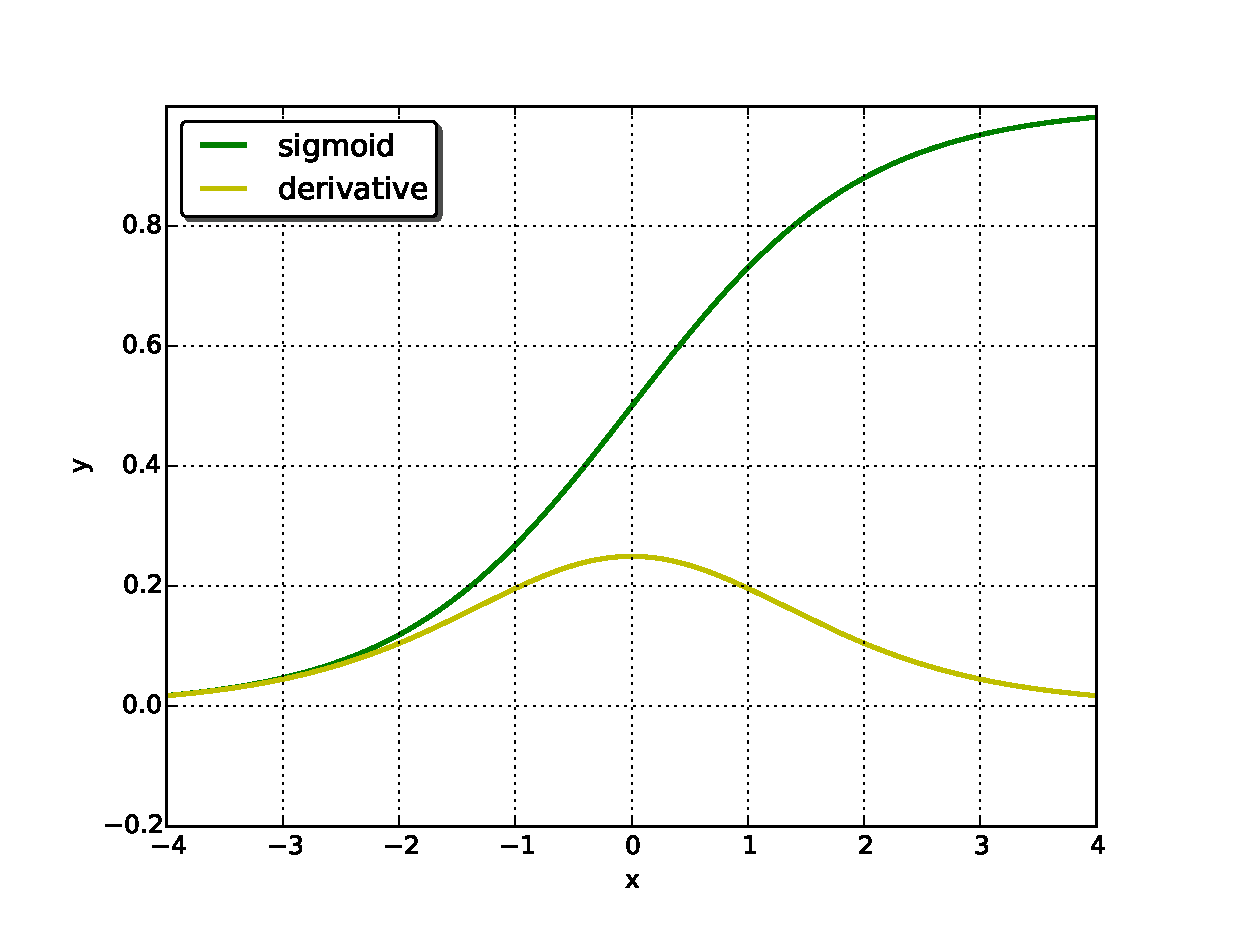
\includegraphics[width=0.9\textwidth]{sigmoid_and_deriv.eps}
  \caption{sigmoid and it's derivative}
\label{sigmoid_plot}
\end{figure}

\paragraph{Tanh}
\begin{align}
 tanh(x)&=\frac{e^x-e^{-x}}{e^x+e^{-x}} \\
 tanh'(x)&= 1 - tanh^2(x)  
\end{align}
As we can see from figure \ref{tanh_plot} tanh (and it's derivative) have a behaviour similar to the sigmoid one; Again we have two saturation region towards
infinity: that's typical of all squashing functions.



\begin{figure}[ht]
  \centering
    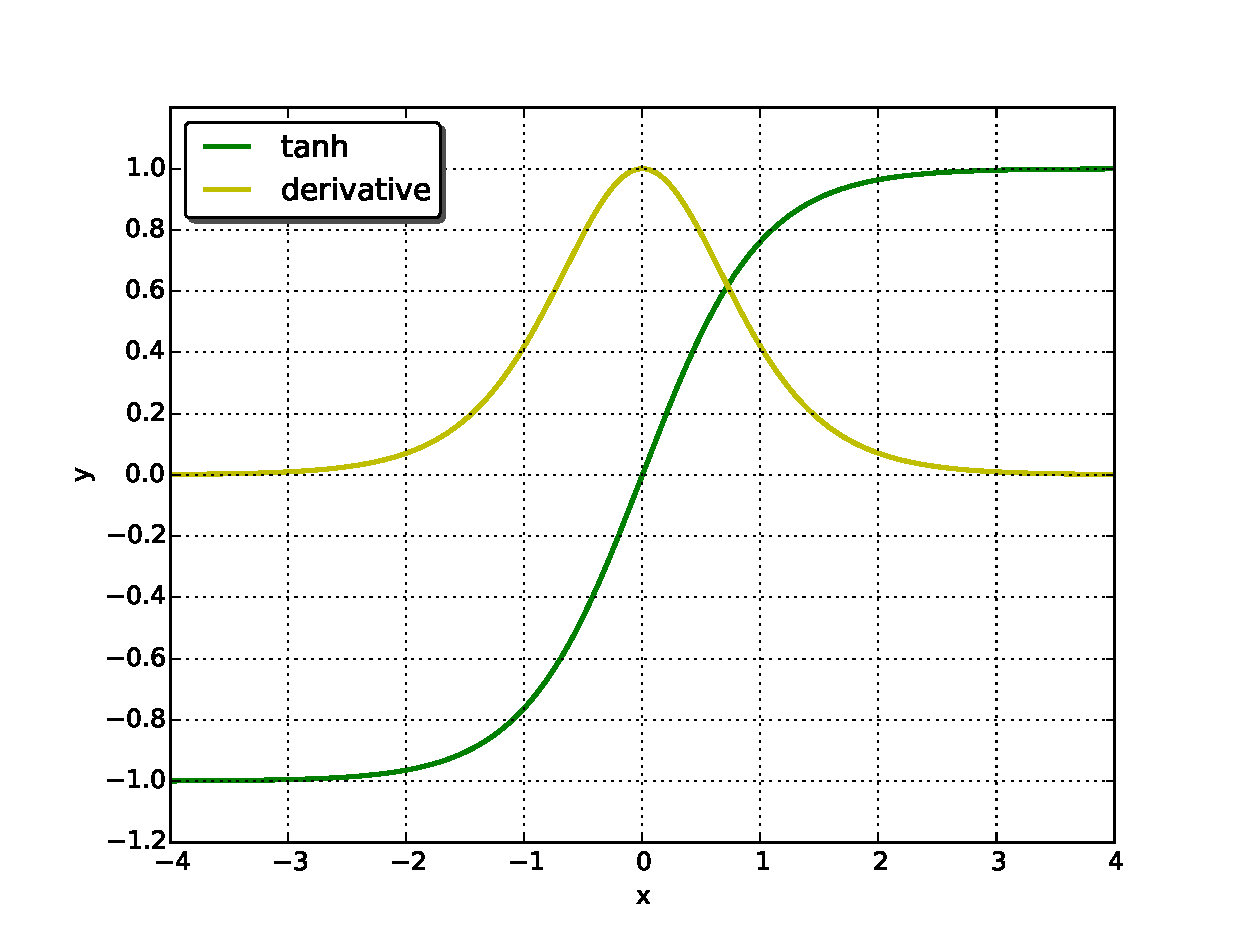
\includegraphics[width=0.9\textwidth]{tanh_and_deriv.eps}
  \caption{tanh and it's derivative}
\label{tanh_plot}
\end{figure}

\paragraph{ReLU}


\begin{align}
  ReLU(x)&=\begin{cases}
    x & \text{if $x>0$}.\\
    0 & \text{otherwise}.
  \end{cases} \\ 
   ReLU'(x)&=\begin{cases}
    1 & \text{if $x>0$}.\\
    0 & \text{otherwise}.
  \end{cases}
\end{align}
ReLU is a bit different from other activation function seen so far: the main difference is that's it's not a squashing function.
As we can see from figure \ref{relu_plot}, ReLU's derivative is the step function; it has only one \textit{saturation} region $(-\infty, 0]$ and a region in which is always takes value one, $(0,+\infty]$
This leads to the fact that we cannot learn to \textit{turn on} a switched off neuron ($x<0$), but we have no \textit{saturation} region toward infinity.

\begin{figure}[ht]
  \centering
    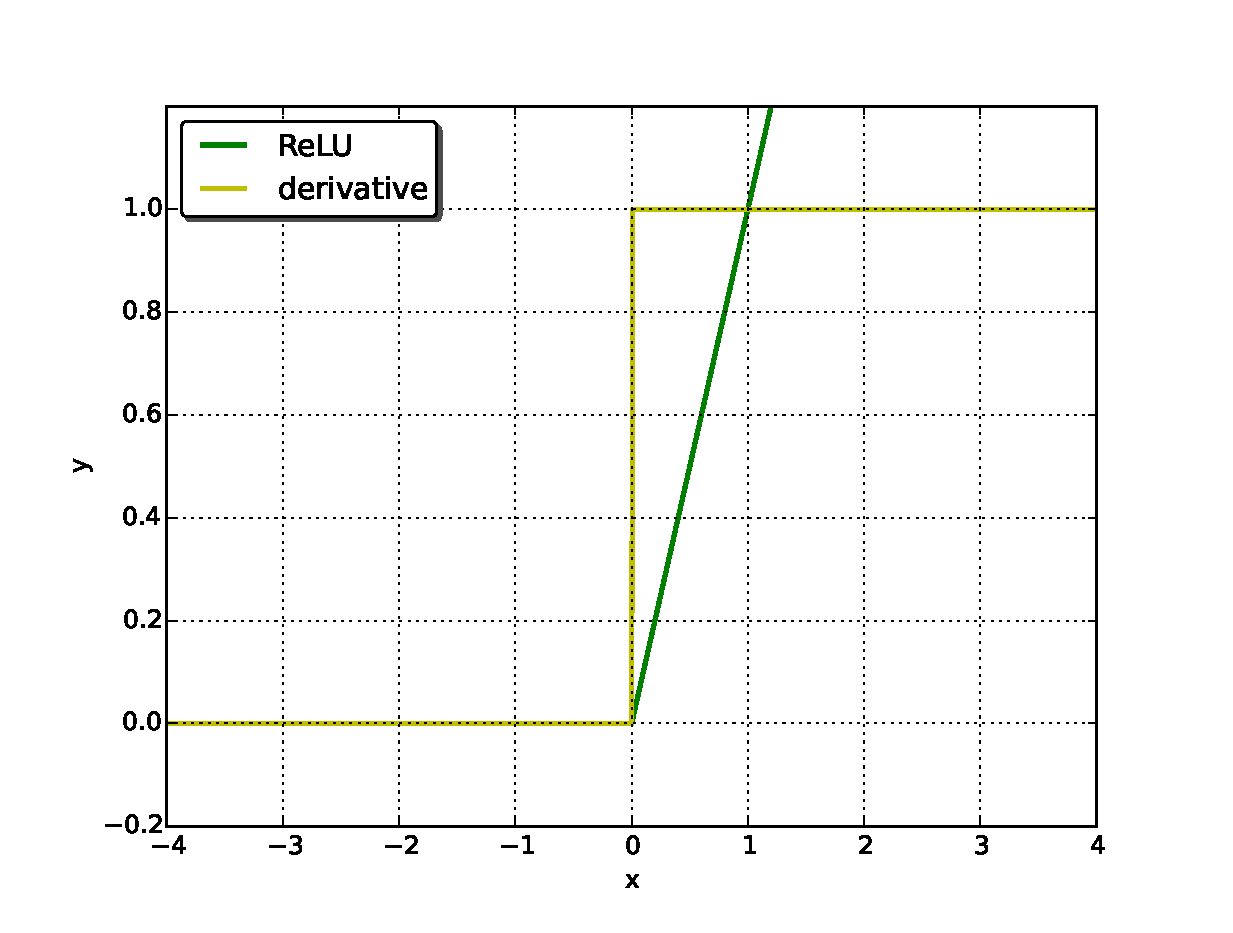
\includegraphics[width=0.9\textwidth]{relu_and_deriv.eps}
  \caption{ReLU and it's derivative}
\label{relu_plot}
\end{figure}

  \section{Stochastic gradient descent: a common framework}
  \label{sec:sgd}
In this section we will describe a framework based on gradient descent optimization method which can be used to train 
neural network of any kind. Such framework constitutes the core of many learning methods used in today's applications. 
Suppose we have a training set of pairs $D=\{\pair{\vec{x}^{(i)}}{\vec{y}^{(i)}}\}$ and a loss function $L(\theta)$ 
where $\theta$ represents all the parameters of the network.

A standard gradient descend would update $\theta$ at each iteration using the gradient computed on the whole training 
set, as shown below.
\begin{equation}
 \theta = \theta - \alpha \nabla_\theta L(\theta).
\end{equation}

This can be very slow or even impractical if the training set is too huge to fit in memory. Stochastic gradient descent (SGD)
overcome this problem taking into account only a part of the training set for each iteration, i.e. the gradient is computed only on a subset $I$ of training examples. 

\begin{equation}
 \theta = \theta - \alpha \nabla_\theta L(\theta; I)
 \label{eq:updateRule}.
\end{equation}

The subset of training examples used for the update is called \textit{mini-batch}. The number of examples for each 
mini-batch is an important hyper-parameter because it affects both the speed of convergence in terms of number of 
iterations and time needed for each iteration. At each iteration new examples are chosen among the training set, so it could, and it always does if we have a finite data-set, happen, that all training set examples get used.
This is not a problem, since we can use the same examples over and over again. Each time we go over the entire training 
set we say we completed and \textit{epoch}. It is not unusual to iterate the learning algorithm for several epochs before converging.

The method is summarized in algorithm \ref{algo:sgd}.

\begin{algorithm}[]
 \KwData{\\
 \Indp
  $D=\{\pair{\vec{x}^{(i)}}{\vec{y}^{(i)}}\}$: training set\\
  $\theta_0$: candidate solution \\
  $m$: size of each mini-batch\\
  }
  
 \KwResult{\\
 \Indp $\theta$: solution
 }
 \BlankLine
 
 $\theta \gets \theta_0$\\
 \While{stop criterion}{
 
 $I$ $\gets$ select $m$ training example $\in D$  \\
 $\alpha \gets$ compute learning rate \\
 $\theta \gets \theta - \alpha \nabla_\theta L(\theta; \pair{\vec{x}^{(i)}}{\vec{y}^{(i)}}, i\in I)$\\
 }
\caption{Stochastic gradient descent}
\label{algo:sgd}
\end{algorithm}

In the following paragraphs we will analyze in more detail each step of the method, surveying the different alternatives 
that can be used.

\paragraph{The stop criterion}

Usually a gradient based method adopts a stop criterion which allows the procedure to stop when close enough to a (local) 
minimum, i.e $\nabla_\theta L(\theta)=0$.  This could easily lead to over-fitting, so is common practice to use a 
cross-validation technique. The most simple approach to cross-validation is to split the training set in two parts, one actually used as a pool of training examples, which will be called \textit{training set}, and the other, called \textit{validation-set}, used to decide when to stop.

Being $D=\{\pair{\vec{x}^{(i)}}{\vec{y}^{(i)}}, i\in(1,M)\}$ a generic subset of the data-set, we can define the \textit{error} on such set in a straightforward manner as 

\begin{equation}
 E_D = \frac{1}{M} \sum_{i=1}^M  L(\vec{x}^{(i)},\vec{y}^{(i)})
\end{equation}

Since training examples are sampled from the training-set, the error on the training-set will always\footnote{This is not actually true; it would in a standard gradient descent, but since we are using stochastic gradient the error could be non monotonic decreasing. However the matter here is that error mainly follow a decreasing path} be decreasing across iterations. The idea behind cross-validation is to compute, and \textit{monitor} the error on the validation set, since it's not guaranteed at all that the error would be decreasing. On the contrary, tough error will generally decrease during the first part of training, it will reach a point when it will start to increase. This is the point when we need to stop training since we are starting to over-fitting. Of course this is an ideal situation, in real applications the validation error could have a more irregular trend, but the idea holds.


\paragraph{Learning rate}

The parameter $\alpha$ in Equation (\ref{eq:updateRule}) is usually referred to as \textit{learning rate}. Of course the strategy employed to compute such learning rate is an important ingredient in the learning method.
The most easy, and often preferred, strategy is that of \textbf{constant learning rate}. The learning rate $\alpha$ becomes another hyper-parameter of the network that can be tuned, but it remains constant, usually a very small value, across all iterations.

Another popular strategy is that of \textbf{momentum} which, in the optimization field is know as the \textit{Heavy 
Ball} method \cite{momentum}.
The main idea behind momentum is to accelerate progress along dimensions
in which gradient consistently point to and to slow down progress along dimensions where the sign of the gradient continues to change. This is done by keeping
track of past parameter updates with an exponential decay as shown in Equation (\ref{eq:momentum}).

\begin{align}
\label{eq:momentum}
v &= \gamma v+ \alpha \nabla_\theta L(\theta; \pair{\vec{x}^{(i)}}{\vec{y}^{(i)}}, i\in I)\\
\theta &= \theta + v
\end{align}

Another way of choosing the learning rate is to fix an initial value and \textbf{annealing} it, at each iteration (or epoch), according to a policy, for instance \textit{exponential} or \textit{linear} decay; the idea behind it being that, initially, when far from a minimum having a larger learning rate causes greater speed and after some iterations when approaching a minimum a smaller learning rate allows a finer refinement.

\textbf{Adaptive} methods, instead, choose the learning rate monitoring the objective function, hence learning rate can be reduced
or increased depending on the need, proving to be a little more versatile than annealing methods. Of course different strategies for detecting when to reduce or increase the learning rate have been devised.

Finally \textbf{line search} which is generally used when working with (non stochastic) gradient descend or when dealing with large batches. For stochastic gradient with small batches other strategies are usually 
preferred.

\paragraph{How to choose batches}

Empirical evidence has been provided that choosing a ``meaningful'' order in which examples are presented to the network can both speed the convergence and yield better solutions. Generally speaking, the network can learn faster if trained first with easier examples and then with examples with gradually increasing difficulty, as humans or animals would do. The idea was introduced by Bengio et al.\cite{curriculumLearning} in 2009, as \textit{curriculum} learning. Experiments on different curriculum strategies can be found in \cite{learningToExecute}.


  \section{The vanishing and exploding gradient problem}
    \label{vanishing_sec}
    We have seen in the previous section that
\begin{equation}
\frac{\partial \vec{a}^t}{\partial \vec{a}^k} = \prod_{i=t-1}^{k}  diag(\sigma'(\vec{a}^i)) \cdot \mat{W}^{rec}
\end{equation}

In an equivalent way with can rewtite the previous equation with respect to a couple of neurons $i$ and $j$

\begin{equation}
\frac{\partial \vec{a}_i^t}{\partial \vec{a}_j^k} = \sum_{q\in P(j)} \sum_{l \in P(q)} \hdots \sum_{h : i \in P(h)} w_{qj} \hdots w_{jh} \cdot \sigma'(a_j^k)\sigma'(a_q^{k+1}) \hdots \sigma'(a_i^{t-1})
\label{expanded_mem}
\end{equation}


Observing the previous equation we can argue that each derivatives it's the sum of $p^{t-k-1}$ terms; each term represents the path cost from neuron $i$ to neuron $j$ in the unfolded network, obviously
there are $p^{t-k-1}$ such paths. If we bind the cost $\sigma'(a_l^t)$ to neuron $l$ in the $t^{th}$ layer in the unfolded network we can read the path cost simply surfing the unfolded network multiply
the weight of each arc we walk through and the cost of each neuron we cross, as we can see from figure \ref{gradient_path_cost}.


\tikzstyle{rnn_style}=[->,shorten >=1pt,auto,node distance=1.5cm,
  thick,
  neuron/.style={circle,fill=white!50,draw,minimum size=0.7cm,inner sep=0pt,font=\sffamily\normalsize},
  missing/.style={circle,fill=white!50,draw=none,minimum size=0.7cm,font=\sffamily\Huge\bfseries},
  label/.style={node distance=1.2cm,rectangle,fill=white!50,draw=none,minimum size=0.7cm,font=\sffamily\normalsize},
  thick_edge/.style={line width=1.2pt},
  thin_edge/.style={dotted, line width=0.5pt},
  weight/.style = {above,sloped,pos=0.3},
  ]
\begin{figure}
 \centering
\begin{tikzpicture}[rnn_style]

  
  \node[neuron]    (x1)[]   {$\sigma_1^t$};
  \node[neuron]    (x2)[right of=x1]   {};
  \node[neuron]    (x3)[right of=x2]   {};
  \node[label]     (xl)[left of=x1] {$t$};
  
  \node[neuron]    (h1)[below of =x1]   {$\hdots$};
  \node[neuron]    (h2)[right of=h1]   {};
  \node[neuron]    (h3)[right of=h2]   {};
  \node[label]     (hl)[left of=h1] {$\hdots$};
  
  \node[neuron]    (y1)[below of=h1]   {};
  \node[neuron]    (y2)[right of=y1]   {};
  \node[neuron]    (y3)[right of=y2]   {$\sigma_3^{k+2}$};
  \node[label]     (yl)[left of=y1] {$k+2$};

  
  \node[neuron]    (z1)[below of=y1]   {$\sigma_1^{k+1}$};
  \node[neuron]    (z2)[right of=z1]   {};
  \node[neuron]    (z3)[right of=z2]   {};
  \node[label]     (zl)[left of=z1] {$k+1$};
  
  \node[neuron]    (w1)[below of=z1]   {};
  \node[neuron]    (w2)[right of=w1]   {$\sigma_2^k$};
  \node[neuron]    (w3)[right of=w2]   {};
  \node[label]     (wl)[left of=w1] {$k$};

  
%   \node[label]      (lu)[left of=u] {$u$};
%   \node[label]      (ll)[left of=z1] {$l$};


  \path[->] (h1) edge [thick_edge] node[weight]{$w_{11}$}  (x1)
	    (h1) edge [thin_edge]   (x2)
	    (h1) edge [thin_edge]   (x3)
	    (h2) edge [thin_edge]  (x1)
	    (h2) edge [thin_edge]   (x2)
	    (h2) edge [thin_edge]   (x3)
	    (h3) edge [thin_edge]  (x1)
	    (h3) edge [thin_edge]   (x2)
	    (h3) edge [thin_edge]   (x3);

  \path[->] (y1) edge [thin_edge]   (h1)
	    (y1) edge [thin_edge]   (h2)
	    (y1) edge [thin_edge]   (h3)
	    (y2) edge [thin_edge]   (h1)
	    (y2) edge [thin_edge]   (h2)
	    (y2) edge [thin_edge]   (h3)
	    (y3) edge [thick_edge] node[weight]{$w_{13}$}   (h1)
	    (y3) edge [thin_edge]   (h2)
	    (y3) edge [thin_edge]   (h3);
  
  
  \path[->] (z1) edge [thin_edge]   (y1)
	    (z1) edge [thin_edge]  (y2)
	    (z1) edge [thick_edge] node[weight]{$w_{31}$}   (y3)
	    (z2) edge [thin_edge]  (y1)
	    (z2) edge [thin_edge]  (y2)
	    (z2) edge [thin_edge]  (y3)
	    (z3) edge [thin_edge]   (y1)
	    (z3) edge [thin_edge]   (y2)
	    (z3) edge [thin_edge]   (y3);
	    
  \path[->] (w1) edge [thin_edge]   (z1)
	    (w1) edge [thin_edge]  (z2)
	    (w1) edge [thin_edge]   (z3)
	    (w2) edge [thick_edge] node[weight]{$w_{12}$}   (z1)
	    (w2) edge [thin_edge]   (z2)
	    (w2) edge [thin_edge]   (z3)
	    (w3) edge [thin_edge]   (z1)
	    (w3) edge [thin_edge]   (z2)
	    (w3) edge [thin_edge]   (z3);

	    


\end{tikzpicture}
\caption{The cost for a path from neuron $2$ at time $k$ to neuron $1$ at time $t$ is $w_{12}w_{31}w_{13}\hdots w_{11}\cdot \sigma_2^k \sigma_1^{k+1}\sigma_3^{k+2} \hdots \sigma_1^{t-1} $ }
\label{gradient_path_cost}
\end{figure}


We can further characterize each path cost noticing that we can separate two components, one that depends only on the weights $w_{qj} \hdots w_{jh}$ and the other that depends both on the weights and the inputs
$\sigma'(a_j^k)\sigma'(a_q^{k}) \hdots \sigma'(a_i^{t-1})$.


\paragraph{Hochreiter Analysis: Weak upper bound}

Let's put $$\sigma'_{max} \triangleq \underset{i=k,...,t-1}{\text{max  }} \{||diag(\sigma'(a^i))||_1\}$$.

We have then:
$$\left\Vert \prod_{i=t-1}^{k}  diag(\sigma'(\vec{a}^i)) \cdot \mat{W}^{rec} \right\Vert_1 <= \prod_{i=t-1}^{k} p \cdot ||diag(\sigma'(\vec{a}^i))||_1 \cdot ||\mat{W}^{rec}||_1 $$
since 
$$||diag(\sigma)\cdot \mat{W}||_1 =
\left\Vert 
\begin{array}{c c c c}
\sigma_1 w_{11} & \sigma_1 w_{12} & \hdots & \sigma_1 w_{1p}  \\
\sigma_1 w_{21} & \sigma_2 w_{22} & \hdots & \sigma_2 w_{2p}  \\
\vdots & \vdots  & \vdots & \vdots  \\
\sigma_p w_{p1} & \sigma_p w_{p2} & \hdots & \sigma_p w_{pp}  \\
\end{array}  
\right\Vert_1
<=p \cdot \sigma_{max} \cdot ||\mat{W}||_1
$$

Hence
\begin{align}
\left\Vert \prod_{i=t-1}^{k}  diag(\sigma'(\vec{a}^i)) \cdot \mat{W}^{rec} \right\Vert_1 & <= p \cdot \big(\sigma'_{max}\cdot ||\mat{W}||_1\big)^{t-k-1} \\
& = p \cdot \tau^{t-k-1}
\end{align}
where $$\tau \triangleq \sigma'_{max}\cdot ||\mat{W}||_1$$

So we have exponential decay if $\tau<1$; We can match this condition assuring that
$$\frac{p\cdot ||w_{max}||}{\sigma_{max}}<1$$ where $w_{max}$ is the maxixum value in the weight matrix.


COMPORTAMENTO SBALIATO STRUTTURALE\\
RELU-NON POSSIAMO IMPARARE AD ACCENDERE \\
MEMORIA\\





  \section{On expressiveness}
  In this section we will investigate the expressive power of neural networks, presenting some results that motivate the use of neural networks as learning
model; we will also show how different architectures leads to different kind of computational power.
 

Maybe the most important result regarding the expressive power of neural networks it's due to Hornik et al. \cite{Hornik89} which basically states
\textit{'Multilayered feed foward networks with at least one hidden layer, using an arbitrary squashing function can approximate virtually any function
of interest to any desired degree of accuracy provided sufficiently many hidden units are available'}.

To give a more formal result we need first to define what \textit{approximate to any degree of accuracy means}, this concept is captured in definition
\ref{dens_compact}
 
\begin{defn}
 A subset S of $\mathbb{C}^n$ (continuoos functions in $\mathbb{R}^n$) is said to be \textit{uniformly dense on compacta in} $\mathbb{C}^n$ if $\forall$
 compact set $K\subset \mathbb{R}^n$ holds: $\forall \epsilon >0$, $\forall g(\cdot) \in \mathbb{C}^n$ $\exists f(\cdot) \in S$ such that 
 $\underset{x \in K}{\text{sup  }} \norm{f(x)-g(x)}<\epsilon$ 
 \label{dens_compact}
\end{defn}

Hornik result is contained in theorem \ref{universal_approx}.
\begin{thm}
 For every activation function $\sigma$, $\forall n\in \mathbb{N}$, feed foward neural
 networks with one hidden layer are a class of functions which is \textit{uniformly dense on compacta in} $\mathbb{C}^n$
\label{universal_approx}.
\end{thm}
Therem \ref{universal_approx} extends also to Borel measurable functions, please see \cite{Hornik89} for more details.


This result implies that FNN are \textit{universal approximators}, this is a strong argument for using such models in machine learning.
It's important to notice, however, that the theorem holds if we have \textit{sufficiently many} units. In praticice the number of units will bounded
by the machine capabilities and by computational time, of course greater the number of units greater will be the learning time. This will limit
the expressiveness of the network to a subset of all measurable functions.

\\\\POGGIO GIROSI?

\\\\RNNs


\chapter{An historical review of proposed solutions}
  
Hochreiter\cite{lstm} in 1991, Bengio et al.\cite{learningIsDifficult} in 1994, and others, observed that gradient in 
deep neural networks tends to either vanish or explode. From then onward several methods have been proposed to 
overcome what is now know as the \textit{exploding/vanishing gradient} problem. We can roughly partition such methods in 
two broad categories.
The approaches of the first kind, the ones we will call \textit{architectural driven}, usually use a simple stochastic gradient descend (SGD) as learning algorithm, and act on the network topology, modifying the way the 
neural units operates, the connections between them or the relationship between layers; the idea of such methods is to 
build networks architectures in which gradient are less likely to vanish, or in other words whose units are able to 
store information for several time steps.

The second approach, which we'll call \textit{learning driven}, instead, focus on the learning algorithm, leaving the 
network architecture untouched. Methods belonging to these categories, either employ learning algorithms different from 
SGD, or they propose modification to the SGD framework.


In the rest of the chapter we will review the most relevant approaches for both the categories.

  \section{Architectural based methods}
  
\subsection{Long short-term memory} 

\textit{Long short-term memory} (LSTM) were proposed (1997) by Hochreiter and Schmidhuber\cite{lstm} as a novel network 
structure to address the vanishing gradient problem, which was first studied by Hochreiter (1991) in his diploma 
thesis, a milestone of deep learning.

The idea behind this structure is to enforce a constant error flow, that is to say, to have constant gradient norm, 
thus preventing the gradient to vanish. This is done by introducing special types of neurons called \textit{memory 
cells} and \textit{gate units}. As we can see by looking at Figure \ref{lstm_neuron}, a memory cell is essentially a 
neuron with a self connection with unitary weight, whose input and output are managed by two multiplicative neurons: 
the gate units.


\tikzstyle{nn_style}=[->,shorten >=1pt,auto,node distance=1.5cm,
  thick,
  neuron/.style={circle,fill=white!50,node distance=1cm,draw,minimum size=0.7cm,font=\sffamily\normalsize},
  missing/.style={circle,font=\sffamily\Large,node distance=0.95cm},
  label/.style={node distance=1.2cm,rectangle,fill=white!50,draw=none,minimum size=0.7cm,font=\sffamily\normalsize},
  layer/.style={rectangle,fill=white!50,draw,minimum width=0.8cm,font=\sffamily\Large},
  loopStyle/.style={in=120,out=60, distance=2.5cm},
  weight/.style = {above,sloped,pos=0.3},]
\begin{figure}[h]
  \centering
  \begin{tikzpicture}[nn_style]

    %horizontal line
    \node[neuron]	(c1)       					{$\times$};
    \node[layer] 	(s_mem)	[right of=c1,	node distance=1.5cm] 	{$\Sigma$};
    \node[neuron]	(mem)	[right of=s_mem,node distance=1.5cm]	{$m_j$};
    \node[layer] 	(h)	[right of=mem,	node distance=1.5cm] 	{$h$};
    \node[neuron]	(c2)	[right of =h,	node distance=1.5cm]	{$\times$};
    \node[label]  	(out)	[right of=c2,	node distance=2.2cm]	{$h_j$};
    
    \path[->] (c1) 	edge []   (s_mem)
	      (s_mem) 	edge []   (mem)
	      (mem) 	edge []   (h)
	      (h) 	edge []   (c2)
	      (c2) 	edge []   (out);
	     
    
    %loop	     
    \path[->] (mem) edge [loop, in=90,out=120, distance=0.8cm, anchor=south ] node [align=center, pos=0.7] 
 {$1$} (s_mem);

    
    %above inputs
    \node[layer] 	(g)	[above of=c1,	node distance=1.5cm] 	{$g$};
    \node[layer] 	(s_in)	[above of=g,	node distance=1.2cm] 	{$\Sigma$};
    \node[missing]	(i2)	[above of=s_in, node distance=1.2cm]	{$\hdots$};
    \node[neuron]	(i3)	[right of=i2, 	node distance=1cm]	{};
    \node[neuron]	(i1)	[left of=i2, 	node distance=1cm]	{};

    
    \path[->] (s_in) 	edge [anchor=west]	node[]{}	(g)
	      (g) 	edge [anchor=west]   	node[]{$a_j$}	(c1)
	      (i1)	edge []   					(s_in) 
      	      (i3)	edge []   					(s_in);
      	      
      	      
    %below gate input unit
    \node[layer] 	(sig_in)	[below of=c1,		node distance=1.5cm] 	{$\sigma$};
    \node[layer] 	(s_gate_in)	[below of=sig_in,	node distance=1cm] 	{$\Sigma$};
    \node[missing]	(gi2)		[below of=s_gate_in, 	node distance=1.2cm]	{$\hdots$};
    \node[neuron]	(gi3)		[right of=gi2, 		node distance=1cm]	{};
    \node[neuron]	(gi1)		[left of=gi2, 		node distance=1cm]	{};

    
    \path[->] (s_gate_in) 	edge [anchor=west]	node[]{}	(sig_in)
	      (sig_in) 		edge [anchor=west]	node[]{$u_j$} 	(c1)
	      (gi1)		edge []   (s_gate_in) 
      	      (gi3)		edge []   (s_gate_in);
      	      
      	      
    %below gate output unit
    \node[layer] 	(sig_out)	[below of=c2,		node distance=1.5cm] 	{$\sigma$};
    \node[layer] 	(s_gate_out)	[below of=sig_out,	node distance=1cm] 	{$\Sigma$};
    \node[missing]	(go2)		[below of=s_gate_out, 	node distance=1.2cm]	{$\hdots$};
    \node[neuron]	(go3)		[right of=go2, 		node distance=1cm]	{};
    \node[neuron]	(go1)		[left of=go2, 		node distance=1cm]	{};

    
    \path[->] (s_gate_out) 	edge [anchor=west]	node[]{}	   (sig_out)
	      (sig_out) 	edge [anchor=west]	node[]{$o_j$}   (c2)
	      (go1)		edge []						   (s_gate_out) 
      	      (go3)		edge []						   (s_gate_out);

    %enclosing rectangle
    \node[rectangle,dashed,fill=none,draw,minimum height=3.2cm,minimum width=8.1cm] at (3.4, 0.5) (memoryCell)	{};
    \node[label]  (memoryLabel)	at(3.5,2.1)	{Memory cell};


      	      
\end{tikzpicture}
\caption{Memory cell and gate units of LSTM network.}
\label{lstm_neuron}
\end{figure}

The memory cell and the gate units behave accordingly to the following:

\begin{align}
&u_j^t = \sigma[\mat{W_u}\cdot\vec{x_t} + \mat{U}_u\cdot\vec{h}_{t-1}]_j \\
&o_j^t = \sigma[\mat{W_o}\cdot\vec{x_t} + \mat{U}_o\cdot\vec{h}_{t-1}]_j \\
&a^t_j\defeq g[\mat{W}\cdot\vec{x_t} + \mat{U}\cdot h_i^t]_j\\
\label{mem_update}
&m_j^t\defeq a_j\cdot u_j^t + (1 \cdot m_j^{t-1})\\
&h_j\defeq h(m_j^t)\cdot o^t_j.
\end{align}


% \begin{equation}
% u^t_j\defeq \sigma(\sum_i w_{ui}\cdot u^{t-1}_j)
% \end{equation}
% \begin{equation}
% o^t_j\defeq \sigma(\sum_i w_{oi}\cdot o^{t-1}_j)
% \end{equation}
% 
% 
% \begin{equation}
% a^t_j\defeq g(\sum_i w_{ij}\cdot \phi_i^t)
% \end{equation}
% \begin{equation}
%  m_j^t\defeq a_j\cdot u_j^t + (1 \cdot m_j^{t-1})
% \label{mem_update}
% \end{equation}
% \begin{equation}
%  \phi_j\defeq h(m_j^t)\cdot o^t_j
% \end{equation}

As we can see from Equation (\ref{mem_update}), the value of the memory cell $m(t)$ remains constant as long as the input 
gate $u$ does not ``open'' causing a ``write'' operation. Similarly the output $o$ of the memory cell, which is 
connected with 
the other neurons of the network, is controlled by an output gate: the memory will have a non zero output only if the 
output gate opens, which we could call a ``read'' operation. As for constant error flow it is ensured because the 
memory cell has only a self-loop with unitary weight.

Memory cells, guarded by gate units can be employed in networks with various topology alongside traditionally 
input, output and hidden units. Another way to look at this kind of architecture is to think of memory cells as units 
able to store one bit of information, even for long periods of time, hence able to learn distant time correlations 
between inputs.

As we have seen these network units are specifically designed to store information, through the use of gates; these 
gates however are no different from other units, apart from the fact they are multiplicative units, hence without 
further precautions, the networks would incur in the same vanishing problem it aimed to resolve. In fact LSTM comes with 
a proper, specifically designed, learning algorithm: essentially errors, i.e. gradients of the loss function, arriving at memory cells inputs are not propagated back in time, only 
the error within the memory cell gets propagated; in other words gradients are truncated taking into account only the 
self-connection of the memory cells and not its other input connections, hence providing constant error flow.
\\\\
LSTM units have proven to be very successful reaching state-of-art results in various tasks and even at the present time (2015), they continue to be largely
employed. In recent implementations however, alongside small modifications, as the introduction of other gates, the LSTM architecture is often used without the original learning algorithm which is often replaced by a standard stochastic gradient descend as done in \cite{lstmGraves}.








   
\subsection{Gated recurrent units}

Gated recurrent units (GRU) were introduced by Cho et al.\cite{gru} in 2014  as units similar to LTSM, with the same purpose, 
but claimed to simpler to compute and implement. A GRU unit $j$ make use of two gate units, $z$, the 
\textit{update} gate, and $r$, the \textit{reset} gate, which are standard neurons.
\begin{align}
 &z_j^t = [\sigma(\mat{W_z}\vec{x_t} + \mat{U}_z\vec{h}_{t-1})]_j\\
 &r_j^t = [\sigma(\mat{W_r}\vec{x_t} + \mat{U}_r\vec{h}_{t-1})]_j.\\
\end{align}
As in LSTM units, the gates manage the access to memory cell, but in GRU they are used a little bit 
differently. The update gate is used to decide how to update the memory cell: the activation value of the cell 
$h_j^{t}$ is a linear interpolation between the previous activation $h_j^{t-1}$ and the candidate activation 
$\tilde{h}_j^t$.
\begin{align}
 &h_j^t \defeq (1-z_j^t)h_j^{t-1} + z_j^t\tilde{h^t_j}\\
  \label{candidateEq}
 &\tilde{h}_j^t = [\sigma(\mat{W}\vec{x_t} + \mat{U}(\vec{r}_t \odot \vec{h}_{t-1})]_j
\end{align}
where $\odot$ symbolize the element-wise product.

As we can see from Equation (\ref{candidateEq}), when the reset gate $r_j^t$ is close to zero, the units acts as if 
reading the first symbol of the input sequence \textit{forgetting} the previous state.

\paragraph{Architecture comparison}
LSTM and GRU present very similarities, the most relevant one being the additive mechanism of update which helps the 
networks to store information during several time step. One difference between the two architectures is, instead, the 
lacking of an output gate in GRU, which hence expose the content of the memory cell without any supervision. In 
\cite{gru_lstm_empirical} Cho et al. compare the two architectures showing how a gated architecture improves the 
performance of a network composed of traditional units; The comparison results obtained were however mixed, and in the 
end they could not demonstrate the superiority of one of the two approaches.

In 2015 an interesting work\cite{architectureMutations} was done  on neural network architectures. The aim of the work was to determine if LSTM or GRU were optimal, or whether a better architecture exists. This was accomplished by comparing thousands of randomly generated architectures using the best hyper-parameter setting for each one. The architectures were generated randomly mutating a given architecture, replacing its activation function nodes, choosing from ReLU, tanh, sigmoid etc., and its operation nodes, with multiplication, subtraction or addition. The result of the experiment is that no one of mutated architectures constantly performed better than LTSM and GRU in all the considered tasks. Moreover the best randomly generated architectures were very similar to the GRU architecture. The conclusion drawn in \cite{architectureMutations}  is that architectures better than LSTM and GRU  either do not exist or are difficult to find. 
  \subsection{Gated feedback recurrent neural networks}

\textit{Gated feedback recurrent neural networks} were proposed in 2015 by  Chung et al. \cite{gatedFeedback} as a novel recurrent network architecture.
Unlike LSTM or GRU where the novelty of the proposal was a new kind of unit, designed to better capture long-term dependencies between inputs, the novelty of this approach is the way the units are arranged. For starters multiple recurrent layer are used, like in a \textit{Stacked RNN}, i.e. the network is composed of several layers, each one of which is connected to all the others; in other words the layers are fully connected. Moreover, unlike traditional stacked RNNs, the feedback connection between different layers is gated by a \textit{global reset gate} which is essentially a logistic unit computed on the current inputs and the previous states of hidden layers. This global reset gates is reminiscent of the gates of LSTM and GRU but it controls the connection between layers not between units: the hidden state values of layer $i$ at time $t-1$ are fed to a lower layer $j$ multiplied by $g^{i\rightarrow j}$.
The gate between layers $i$ and $j$ is computed as:
\begin{equation}
g^{i\rightarrow j} \defeq \sigma(\vec{w}_g^{i\rightarrow j} \cdot \vec{h_t}^{j-1} + \vec{u}_g^{i\rightarrow j} \cdot \vec{h}^*_{t-1})
\end{equation}
where $\vec{w}_g^{i\rightarrow j}$ and $\vec{u}_g^{i\rightarrow j}$ are the weights of the links between the gate and the input and the hidden states of all layers at time-step $t-1$ respectively; for $j=1$,  $\vec{h}_t^{j-1}=\vec{x}_t $  and $\vec{h^*_{t-1}}$ represents all the hidden states at time $t-1$.

The idea behind this architecture is to encourage each recurrent layer to work at different timescales, hence capturing both long-term and short-term dependencies. In addition, the units composing the layers, can be traditional sigmoidal units but also LSTM or GRU, hence benefiting from both the strength of these kind of units and the global gate mechanism. In \cite{gatedFeedback} the architecture is evaluated against traditional and stacked RNNs with both LSTM and GRU units: gated feedback networks are shown to offer better performance and accuracy in several challenging tasks.


\tikzstyle{rnn_style}=[->,shorten >=1pt,auto,node distance=1.5cm,
  thick,
  neuron/.style={circle,fill=white!50,draw,node distance = 1cm, minimum size=0.7cm,font=\sffamily\Large\bfseries},
  gate/.style={circle,fill=white!50,draw,node distance = 1cm,font=\sffamily\small\bfseries},
  missing/.style={rectangle,fill=white!50,node distance =1cm,draw=none,minimum size=0.7cm,font=\sffamily\Huge\bfseries},
  label/.style={node distance=1.2cm,rectangle,fill=white!50,draw=none,minimum size=0.7cm,font=\sffamily\normalsize},
  layer/.style={rectangle,fill=white!50,draw,minimum width=4cm,minimum height=0.5cm, font=\sffamily\normalsize},
  gateEdge/.style={dotted},]
\begin{figure}
 \centering
\begin{tikzpicture}[rnn_style]
  
  \node[layer] (l1)[] {$L_1$};
  \node[missing] (l2)[above of=l1,node distance=1.2cm]{$\hdots$};
  \node[layer] (l3)[above of=l2,node distance=1.2cm] {$L_3$};
  \node[layer] (l4)[above of=l3,node distance=1.2cm] {$L_4$};
  
  \node[label] (x) [below of=l1, node distance=1.2cm]{$\vec{x}$};
  \node[label] (y) [above of=l4, node distance=1.2cm]{$\vec{y}$};

  
    \path[->] (l1) edge 	[] node[]{}   	(l2)
	    (l2) edge 	[]   		(l3)
	    (l3) edge	[]		(l4)
	    (x) edge[]			(l1)
	    (l4) edge[]			(y);
  
  \node[gate] (g44)[left of=l4, node distance =3cm]{$g_{44}$};
  \node[gate] (g43)[left of=l3, node distance =3cm]{$g_{43}$};
  \node[gate] (g41)[left of=l1, node distance =3cm]{$g_{41}$};
  \node[gate] (g33)[right of=l3, node distance =3cm]{$g_{33}$};
  \node[gate] (g31)[right of=l1, node distance =3cm]{$g_{31}$};
  \node[gate] (g11)[below of=g31, node distance =1.3cm]{$g_{11}$};
  
      \path[->] (g44) edge[gateEdge]   		(l4)
		(l4.north)  edge[gateEdge,bend right=50] (g44.north)
		(l4.north)  edge[gateEdge,bend right=90,distance=2.8cm] (g43.west)
		(g43) edge[gateEdge]		(l3)
		(l4.north)  edge[gateEdge,bend right=100, distance =4.5cm] (g41.west)
		(g41) edge[gateEdge]		(l1)
		(l3.east)  edge[gateEdge,bend left=50, anchor=east]	(g33)
		(g33) edge[gateEdge]		(l3)
		(l3.east)  edge[gateEdge,bend left]	(g31.north)
		(g31) edge[gateEdge]		(l1)
		(l1.east) edge[gateEdge, bend left]		(g11.north)
		(g11) edge[gateEdge, bend left]		(l1);

\end{tikzpicture}
\caption{Gated feedback architecture. Only connections between layers are shown, dotted when trough gates.}
\label{fig:gated}
\end{figure}


  \section{Learning based methods}
  \subsection{Preserve norm by regularization and gradient clipping} 

In 2013 Pascanu \cite{pascanu} proposed a regularization term $\Omega$ for the loss function $L(\theta)$ which should address the vanishing gradient problem.
The objective function hence become:
\begin{equation}
 \tilde{L}(\theta) \defeq L(\theta) + \lambda\Omega(\theta)
\end{equation}

Such a term represents a preference for solutions such that back-propagated gradients preserves norm in time.
\begin{equation}
\Omega = \sum_t \left( \frac{\norm{ \frac{\partial L}{\partial \vec{h}_{t+1}} \cdot \frac{\partial \vec{h}_{t+1}}{\partial \vec{h}_t} }}{\norm{\frac{\partial L}{\partial \vec{h}_{t+1}}}} -1  \right)^2 
\label{eq:pascanuReg}
\end{equation}

As we can see from equation \ref{eq:pascanuReg} the regularization term forces $\frac{\partial \vec{h}_{t+1}}{\partial \vec{h}_t}$ to preserve norm in the relevant direction of the error $\frac{\partial L}{\partial \vec{h}_{t+1}}$.

The intuition behind this technique is that $\frac{\partial \vec{h}_{t}}{\partial \vec{h}_k}$ measure the dependence of outputs at time $t$ on the previous time steps $t-1,...k$. In \cite{pascanu} is argued that even though some precedent inputs $k<t$ will be irrelevant for the prediction of time time $t$, the network cannot learn to ignore them unless there is an error signal; hence it's a good idea to force the network to increase $\frac{\partial \vec{h}_{t}}{\partial \vec{h}_k}$, even at the expense of greater error of the loss function $L(\theta)$, and then wait for it to learn to ignore these inputs.

As for the exploding vanishing gradient, in \cite{pascanu} is argued that a simple method called \textit{gradient clipping}, first used by Mikolov\cite{clippingMikolov}, can be effective against exploding gradient. The method, shown in algorithm \ref{algo:gradClipping}, simply consists in rescale the gradient norm when it goes over a threshold.

\begin{algorithm}[]
$\vec{g} \gets \nabla_{\theta} L$\\
\If{$\norm{\vec{g}} \geq threshold $}{$\vec{g} \gets \frac{threshold}{\norm{\vec{g}}} \vec{g}$}
\caption{Gradient clipping}
\label{algo:gradClipping}
\end{algorithm}

A drawback of such an approach is the introduction of another hyper-parameter, the threshold, however in \cite{pascanu} is said that a good heuristic
is to choose a value from half to ten time the average gradient norm over a sufficiently large number of updates.
The algorithm can be described also in term of adjusting the learning rate monitoring the gradient. Our understanding is that such escamotage is not necessary at all when, for instance, using a line search algorithm for setting the learning rate.

% \chapter{Some results}
%   \section{Vanishing gradient solutions}
%   In section \ref{vanishing_sec} were established some weak bounds on the weight matrix $\mat{W}^{rec}$ whose crossing entails the arising of
the vanishing gradient problem.

It would be nice to find some lower bounds on the weight matrix which don't allow an exponential decay of long term components. However since activation
functions can all have zero value, we cannot establish any lower bound different from zero.

However what we are really interested in is the cost of the paths which cross \textit{active} neurons because, structurally, \textit{switched off} neurons don't
contribute to the gradient. Formally we define


\begin{defn}{Active neuron}
A neuron $j$ is said to be active if $$\sigma(a_j)>\tau$$
 
\end{defn}






To overcame this problem we return to the previously introduced graph formulation where we consider each component 
$\frac{\partial \vec{a}_i^t}{\partial \vec{a}_j^k}$ as the sum path cost.



\begin{equation} 
\frac{\partial \vec{a}_i^t}{\partial \vec{a}_j^k} = \sum_{q\in P(j)} \sum_{l \in P(q)} \hdots \sum_{h : i \in P(h)} w_{qj} \hdots w_{jh} \cdot \sigma'(a_j^k)\sigma'(a_q^{k+1}) \hdots \sigma'(a_i^{t-1})
\label{expanded_mem}
\end{equation}

\appendix
\chapter{Notation}

Let $F:\mathbb{R}^N \rightarrow \mathbb{R^M}$ be defined by
\begin{equation}
F(\vec{x}) = (f_1(\vec{x}),f_2(\vec{x}),\cdots,f_M(\vec{x}))) \text{    for some  } f_i:\mathbb{R}^N \rightarrow \mathbb{R}
\end{equation}

\begin{defn}[Derivative with respect to a vector]
 We define the derivative of $F(x(\vec{w}))$ with respect to a vector $\vec{w}$ of $p$ elements as the $M \times p$ matrix
\begin{equation}
\frac{\partial F}{\partial \vec{w}} \triangleq
\begin{bmatrix}
   \frac{\partial f_1}{\partial \vec{w}_1}    & \frac{\partial f_1}{\partial \vec{w}_2}                & \cdots      & \cdots       & \frac{\partial f_1}{\partial \vec{w}_p}  \\
   \frac{\partial f_2}{\partial \vec{w}_1}    & \frac{\partial f_2}{\partial \vec{w}_2}                & \cdots      & \cdots       & \frac{\partial f_2}{\partial \vec{w}_p}  \\
   \vdots                & \vdots           & \vdots      & \vdots       &\vdots\\
   \frac{\partial f_M}{\partial \vec{w}_1}    & \frac{\partial f_M}{\partial \vec{w}_2}                & \cdots      & \cdots       & \frac{\partial f_M}{\partial \vec{w}_p}
\end{bmatrix}
\end{equation}
\end{defn}


\begin{defn}[Derivative with respect to a matrix]
We define the derivative of $F(x(\mat{W}))$ with respect to a vector $\mat{W}$, being $W_j$ the $j^{th}$ column of a $p\times m$ matrix $W$ as the $M\times (p \cdot m )$ matrix:
\begin{equation}
\frac{\partial F}{\partial \mat{W}} \triangleq
\left[
\begin{array}{c|c|c|c}
\frac{\partial F}{W_1} & \frac{\partial F}{W_2} & \cdots & \frac{\partial F}{W_m} \\
\end{array}
\right]
\end{equation}
\end{defn}







\newpage
% \nocite{*}		 % Mostra in bibliografia anche gli oggetti non citati 
\bibliography{biblio}{}
\bibliographystyle{plain}


\end{document}     